% Bien dich bang XeLaTeX; sua thong tin bia va lien ket nop bai ben duoi.
\documentclass[12pt,a4paper]{article}
\usepackage{fontspec}
\IfFontExistsTF{Times New Roman}{\setmainfont{Times New Roman}}{%
  \IfFontExistsTF{Liberation Serif}{\setmainfont{Liberation Serif}}{\setmainfont{TeX Gyre Termes}}}
\IfFontExistsTF{DejaVu Sans}{\setsansfont{DejaVu Sans}}{\setsansfont{TeX Gyre Heros}}
\IfFontExistsTF{DejaVu Sans Mono}{\setmonofont{DejaVu Sans Mono}[Scale=0.82]}{\setmonofont{Latin Modern Mono}[Scale=0.9]}
\usepackage{polyglossia}
\setdefaultlanguage{vietnamese}
\usepackage[left=3cm,right=2cm,top=2.4cm,bottom=2.4cm,headheight=16pt]{geometry}
\usepackage{amsmath}
\usepackage{graphicx}
\usepackage{booktabs,tabularx,array,makecell}
\usepackage{xcolor}
\usepackage{listings}
\usepackage{caption}
\usepackage{enumitem}
\usepackage{setspace}
\usepackage{fancyhdr}
\usepackage{placeins}
\usepackage[unicode,hidelinks]{hyperref}
\usepackage{xurl}
\graphicspath{{figures/}}
\onehalfspacing
\setlength{\parindent}{1.2em}
\setlength{\parskip}{3pt}
\setlength{\emergencystretch}{2em}
\renewcommand{\arraystretch}{1.18}
\newcolumntype{Y}{>{\raggedright\arraybackslash}X}
\captionsetup{font=small,labelfont=bf,justification=centering}
\setlist[itemize]{nosep,leftmargin=1.5em}
\setlist[enumerate]{nosep,leftmargin=1.8em}
\definecolor{codebg}{RGB}{246,247,249}
\definecolor{codeframe}{RGB}{190,195,203}
\lstset{basicstyle=\ttfamily\footnotesize,backgroundcolor=\color{codebg},
 frame=single,rulecolor=\color{codeframe},breaklines=true,
 breakatwhitespace=false,columns=fullflexible,keepspaces=true,
 showstringspaces=false,tabsize=2,aboveskip=8pt,belowskip=8pt}
\newcommand{\code}[1]{\texttt{\detokenize{#1}}}

% Thong tin ca nhan: thay cac chuoi trong ngoac vuong.
\newcommand{\tenTruong}{[Tên trường]}
\newcommand{\tenKhoa}{[Tên khoa / bộ môn]}
\newcommand{\tenHocPhan}{[Tên học phần]}
\newcommand{\tenGiangVien}{[Họ tên giảng viên]}
\newcommand{\tenSinhVien}{[Họ tên sinh viên]}
\newcommand{\maSinhVien}{[Mã sinh viên]}
\newcommand{\tenLop}{[Tên lớp]}
\newcommand{\diaDiem}{[Địa điểm]}
\newcommand{\linkGithub}{[Bổ sung liên kết GitHub]}
\newcommand{\linkVideo}{[Bổ sung liên kết Google Drive]}

\pagestyle{fancy}
\fancyhf{}
\fancyhead[L]{\small TurtleBot 4 -- SLAM Toolbox -- Nav2}
\fancyhead[R]{\small \maSinhVien}
\fancyfoot[C]{\thepage}
\hypersetup{pdftitle={Báo cáo thực hành 04: TurtleBot 4, SLAM và Nav2},
 pdfsubject={ROS 2 Jazzy và Gazebo Harmonic}}

\begin{document}
\hypersetup{pageanchor=false}
\begin{titlepage}
\centering
{\large\bfseries \tenTruong\par}
\vspace{0.25cm}
{\large\bfseries \tenKhoa\par}
\vspace{1.5cm}
{\Large\bfseries BÁO CÁO BÀI THỰC HÀNH 04\par}
\vspace{0.9cm}
{\LARGE\bfseries MÔ PHỎNG TURTLEBOT 4,\par}
\vspace{0.2cm}
{\LARGE\bfseries XÂY DỰNG BẢN ĐỒ BẰNG\par}
{\LARGE\bfseries SLAM TOOLBOX VÀ ĐIỀU HƯỚNG\par}
{\LARGE\bfseries TỰ ĐỘNG VỚI NAV2\par}
\vspace{1.5cm}
\begin{tabular}{ll}
Học phần: & \tenHocPhan \\
Giảng viên hướng dẫn: & \tenGiangVien \\
Sinh viên thực hiện: & \tenSinhVien \\
Mã sinh viên: & \maSinhVien \\
Lớp: & \tenLop \\
\end{tabular}
\vfill
{\large \diaDiem, tháng 10 năm 2026\par}
\end{titlepage}

\pagenumbering{arabic}
\hypersetup{pageanchor=true}
\tableofcontents
\newpage

\section{Tổng quan đề tài và cấu trúc chương trình}
\subsection{Mục tiêu bài thực hành}
Bài thực hành triển khai TurtleBot 4 trong môi trường mô phỏng để thực hiện
quy trình từ kiểm tra robot đến xây dựng bản đồ, định vị và điều hướng tự động.
Giai đoạn đầu xác nhận dữ liệu LiDAR, odometry, hệ tọa độ và khả năng nhận lệnh
vận tốc. Sau đó robot được điều khiển bằng bàn phím để khảo sát môi trường;
SLAM Toolbox kết hợp các lần quét với thông tin chuyển động để tạo bản đồ.
Bản đồ được lưu, nạp lại cho AMCL và sử dụng làm cơ sở điều hướng với Nav2.

Các yêu cầu chính của bài gồm:
\begin{enumerate}
\item Khởi chạy robot trong Gazebo; kiểm tra \code{/scan}, \code{/odom},
\code{/cmd_vel} và hiển thị robot, cảm biến trên RViz2.
\item Khảo sát phần lớn khu vực có thể di chuyển; tạo bản đồ thể hiện tường,
hành lang và vật cản chính; lưu hai file YAML và PGM.
\item Dừng SLAM, khởi động lại trong cùng môi trường và định vị trên bản đồ đã lưu.
\item Gửi ba goal ở các khu vực khác nhau; robot tự lập kế hoạch và di chuyển,
không điều khiển thủ công sau khi gửi goal và không va chạm.
\end{enumerate}

\subsection{Môi trường thực hiện}
Hệ thống sử dụng Ubuntu 24.04, ROS 2 Jazzy và Gazebo Harmonic, thay cho cấu
hình Humble/Fortress của một số tài liệu và báo cáo tham khảo. Robot sử dụng
mô hình TurtleBot 4 Standard; world mặc định của các launch là \code{depot}.
Simulator và các thành phần ROS được tái sử dụng từ package chính thức
\cite{tb4sim,tb4source}.

\begin{table}[htbp]
\centering\small
\caption{Môi trường và sản phẩm của dự án.}\label{tab:environment}
\begin{tabularx}{\textwidth}{p{0.31\textwidth}Y}
\toprule
Thành phần & Giá trị \\
\midrule
Hệ điều hành & Ubuntu 24.04 \\
ROS 2 / Python & Jazzy / Python hệ thống 3.12 \\
Gazebo & Harmonic, gz-sim 8; phiên kiểm tra ban đầu dùng 8.11.0 \\
Robot / world & TurtleBot 4 Standard / \code{depot} \\
Workspace / package & \code{~/tb4_ws} / \code{turtlebot4_slam_nav} \\
Bản đồ được cung cấp & \code{depot_02.yaml} và \code{depot_02.pgm} \\
Công cụ quan sát & RViz2, ROS 2 CLI và giao diện Gazebo \\
\bottomrule
\end{tabularx}
\end{table}

\subsection{Cấu trúc và tổ chức chương trình}
Package của bài đóng vai trò tổ chức cách chạy và lưu các sản phẩm thực nghiệm,
không xây dựng lại simulator, controller hoặc thuật toán SLAM/Nav2. Các file
launch include thành phần chính thức theo từng chế độ. Cấu trúc chính như sau:
\begin{lstlisting}
turtlebot4_slam_nav/
|-- launch/
|   |-- simulation.launch.py
|   |-- mapping.launch.py
|   |-- localization.launch.py
|   `-- navigation.launch.py
|-- turtlebot4_slam_nav/
|   |-- launch_helpers.py
|   `-- map_utils.py
|-- config/fastdds_local.xml
|-- rviz/
|-- scripts/
|   |-- env.sh
|   `-- save_map.sh
|-- maps/depot_02.yaml, depot_02.pgm
|-- package.xml
|-- setup.py
`-- README.md
\end{lstlisting}

Bốn chế độ thay thế nhau: simulation chỉ kiểm tra robot; mapping bổ sung
SLAM Toolbox; localization dùng map server và AMCL; navigation bổ sung Nav2.
Trước khi chuyển chế độ phải dừng launch cũ để tránh trùng simulator và node.
Trong mapping, SLAM cung cấp TF từ map đến odom; trong localization/navigation,
AMCL đảm nhiệm biến đổi này. Hai nguồn đó không được chạy đồng thời.
Các node xử lý dữ liệu mô phỏng sử dụng \code{use_sim_time=true}.

\FloatBarrier
\section{Các thành phần chính và kiến trúc hệ thống}
\subsection{Package, node, topic và action}
Các thành phần của hệ thống được tổng hợp trong Bảng~\ref{tab:components}.
Gazebo sinh dữ liệu và mô phỏng chuyển động; ROS--Gazebo bridge chuyển dữ liệu
sang ROS 2 và đưa lệnh điều khiển trở lại simulator. Nhờ đó, SLAM, AMCL, Nav2
và RViz làm việc với các topic và TF của ROS 2.

\begin{table}[htbp]
\centering\small
\caption{Vai trò của các thành phần chính.}\label{tab:components}
\begin{tabularx}{\textwidth}{p{0.35\textwidth}Y}
\toprule
Package / node & Chức năng \\
\midrule
\code{turtlebot4_gz_bringup}, \code{ros_gz_bridge} & Khởi tạo mô phỏng, spawn robot và nối dữ liệu/lệnh Gazebo--ROS. \\
\code{slam_toolbox} & Tạo occupancy map từ scan và TF; cung cấp TF map--odom khi mapping. \\
\code{map_server}, \code{amcl} & Đọc map đã lưu và ước lượng pose của robot. \\
\code{planner_server}, \code{controller_server}, \code{bt_navigator} & Lập đường đi, tính điều khiển và quản lý navigation goal. \\
\code{velocity_smoother}, \code{collision_monitor} & Xử lý lệnh vận tốc trước khi chuyển tới robot. \\
\code{motion_control}, \code{diffdrive_controller} & Tiếp nhận lệnh và điều khiển chuyển động robot mô phỏng. \\
\code{rviz2}, \code{teleop_twist_keyboard} & Quan sát, đặt pose/goal và điều khiển khảo sát bằng bàn phím. \\
\bottomrule
\end{tabularx}
\end{table}

Các topic quan trọng là \code{/scan} (LaserScan), \code{/odom} (Odometry),
\code{/cmd_vel} (TwistStamped), \code{/clock} (thời gian mô phỏng),
\code{/map} (OccupancyGrid), \code{/tf}, \code{/tf_static},
\code{/amcl_pose} và \code{/plan}. Goal được gửi qua action
\code{/navigate_to_pose}, có kiểu \code{nav2_msgs/action/NavigateToPose}.
Đặc biệt, trong Jazzy đang cài, \code{/cmd_vel} nhận
\code{geometry_msgs/msg/TwistStamped}; teleop phải bật tùy chọn
\code{stamped:=true}.

\subsection{Luồng thực hiện tổng thể}
Hình~\ref{fig:architecture} biểu diễn quan hệ giữa hai giai đoạn: tạo bản đồ
và sử dụng bản đồ. Trong khảo sát, dữ liệu scan và TF đi vào SLAM Toolbox.
Map Saver lưu occupancy map thành YAML/PGM. Sau khi dừng SLAM và khởi động
lại cùng world, map server nạp bản đồ, AMCL định vị và Nav2 tính lệnh điều khiển.
Các nhánh trong sơ đồ thể hiện việc tái sử dụng dữ liệu ở những phiên khác nhau,
không có nghĩa SLAM và AMCL cùng chạy trong một phiên.

\begin{figure}[htbp]
\centering
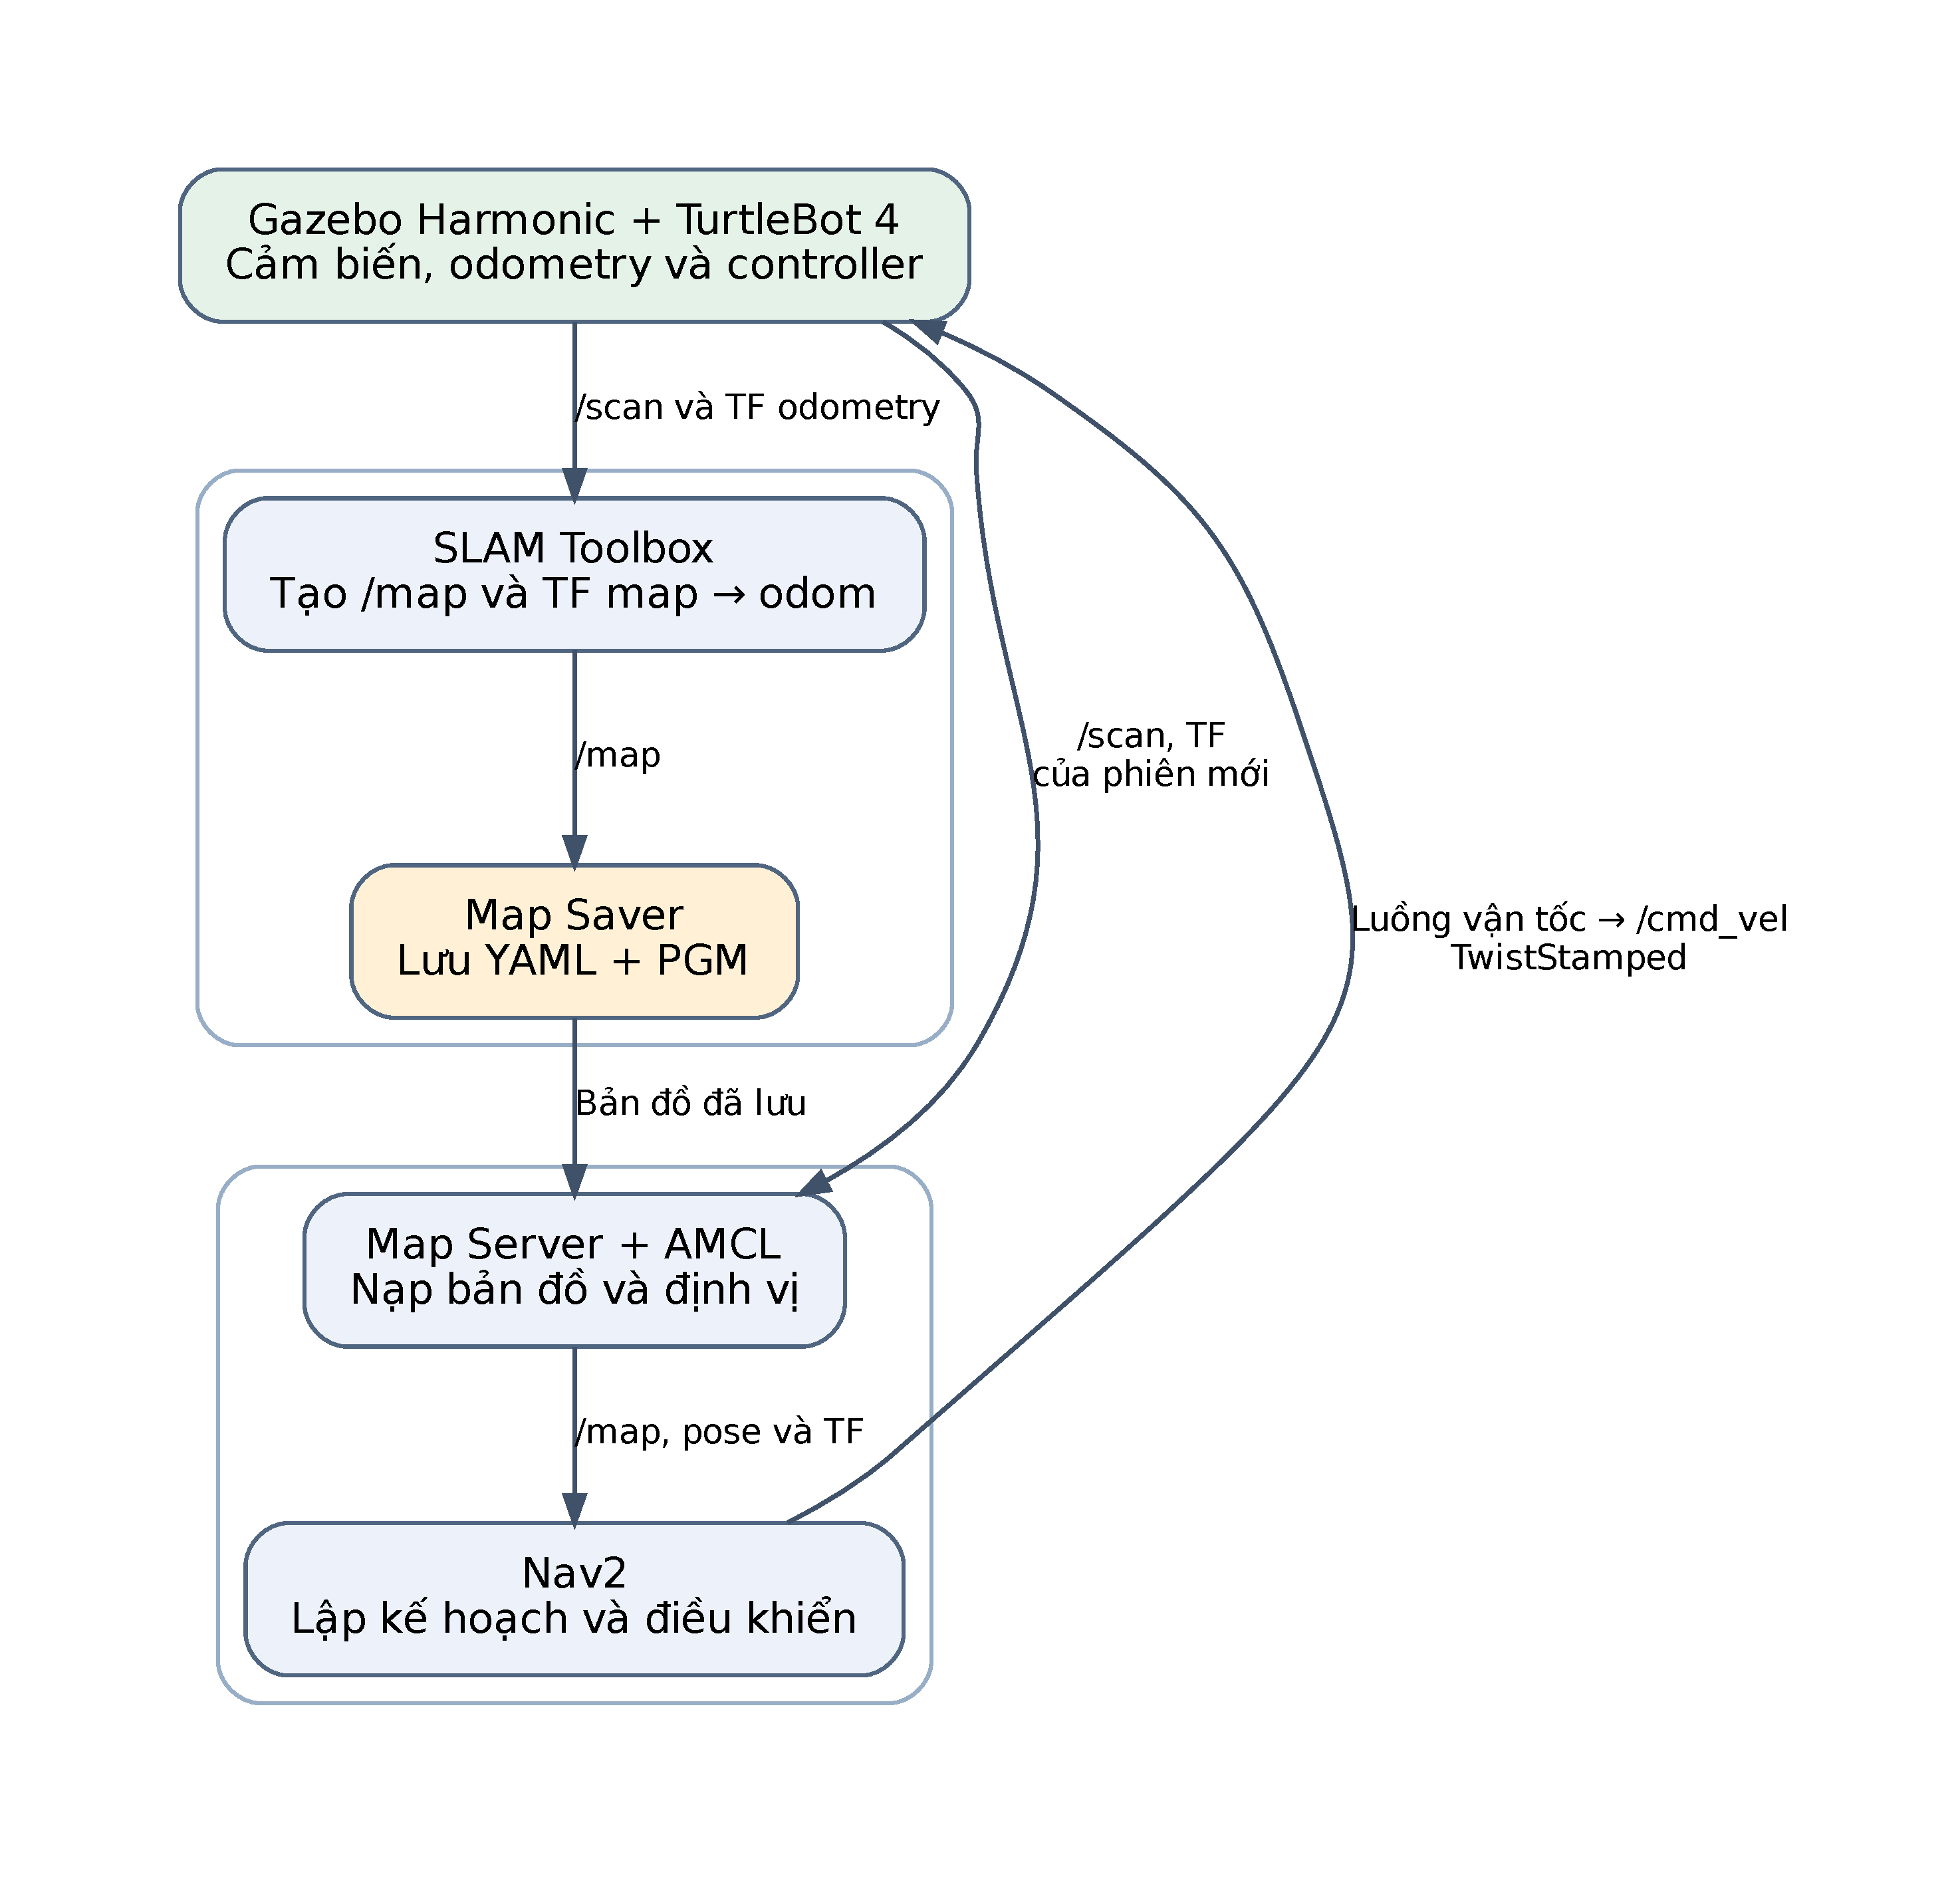
\includegraphics[width=0.85\textwidth,height=0.53\textheight,keepaspectratio]{01_tong_the.pdf}
\caption{Luồng dữ liệu tổng thể từ mapping, lưu bản đồ đến localization và navigation.}
\label{fig:architecture}
\end{figure}

\FloatBarrier
\section{Mô phỏng TurtleBot 4 và kiểm tra hoạt động}
\subsection{Khởi chạy mô phỏng}
Các terminal của bài source script môi trường để dùng Python hệ thống,
ROS 2 Jazzy và cùng ROS domain/Gazebo partition. Script chỉ thay đổi môi
trường của terminal hiện tại. Sau khi build package, chạy simulation:
\begin{lstlisting}
source ~/tb4_ws/src/turtlebot4_slam_nav/scripts/env.sh
cd ~/tb4_ws
/usr/bin/python3 -m colcon build --symlink-install \
  --packages-select turtlebot4_slam_nav
source install/local_setup.bash
ros2 launch turtlebot4_slam_nav simulation.launch.py \
  world:=depot gui_render_engine:=ogre2
\end{lstlisting}

Launch sử dụng world và mô hình robot chính thức. Server và GUI Gazebo được
chạy riêng để việc đóng hoặc lỗi GUI không tự kết thúc server. RViz ở chế độ
simulation dùng fixed frame \code{odom}, vì chưa có hệ tọa độ map.
Sau khi world tải xong, kiểm tra Gazebo đang Play và \code{/clock} có dữ liệu.

\subsection{Kiểm tra LiDAR và odometry}
LiDAR xuất bản \code{sensor_msgs/msg/LaserScan} trên \code{/scan}, gồm timestamp,
frame, góc quét và khoảng cách. Các lệnh kiểm tra cơ bản là:
\begin{lstlisting}
ros2 topic echo /clock rosgraph_msgs/msg/Clock --once
ros2 topic info /scan -v
ros2 topic echo /scan sensor_msgs/msg/LaserScan \
  --once --field header --qos-reliability best_effort
ros2 topic echo /scan sensor_msgs/msg/LaserScan \
  --once --field ranges --qos-reliability best_effort
ros2 topic hz /scan
\end{lstlisting}

Phép kiểm tra khi triển khai ghi nhận scan 640 mẫu. Frame của scan là
\path{turtlebot4/rplidar_link/rplidar}. Trong một mẫu dữ liệu depot đã lưu log,
khoảng cách hữu hạn nhỏ nhất xấp xỉ 1.482 m và lớn nhất xấp xỉ 11.937 m.
Đây là giá trị của một lần kiểm tra, không phải giới hạn tầm đo của sensor.
Các phép đo khác nhau theo tia cho thấy scan không còn bị cố định toàn bộ ở
0.164 m như hiện tượng gặp với sensor engine Ogre trong phiên thử ban đầu.

Topic \code{/odom} có kiểu \code{nav_msgs/msg/Odometry}, chứa pose và vận tốc
trong hệ tọa độ odom. Có thể theo dõi pose liên tục khi teleop:
\begin{lstlisting}
ros2 topic info /odom -v
ros2 topic echo /odom nav_msgs/msg/Odometry --once --field header
ros2 topic echo /odom nav_msgs/msg/Odometry --field pose.pose
\end{lstlisting}

Ảnh terminal đã cung cấp có frame odom, tọa độ gần gốc và quaternion gần
$(0,0,0,1)$; các pose liên tiếp gần như không thay đổi, phù hợp với trạng thái
đứng yên. Ảnh này chứng minh có dữ liệu odometry tại thời điểm chụp nhưng chưa
minh họa được sự thay đổi khi di chuyển. Một ảnh đo tần số khác hiển thị khoảng
15.2 Hz, song không thấy lệnh gọi/tên topic nên không gán kết quả đó riêng cho
scan hoặc odom.

\subsection{Undock, teleoperation và kiểm tra lệnh vận tốc}
Trước khi lái, kiểm tra trạng thái dock. Nếu robot còn dock, sử dụng action
Create 3 để undock và chờ kết quả thành công:
\begin{lstlisting}
ros2 topic echo /dock_status irobot_create_msgs/msg/DockStatus --once
ros2 action send_goal /undock irobot_create_msgs/action/Undock \
  '{}' --feedback
ros2 run teleop_twist_keyboard teleop_twist_keyboard --ros-args \
  -p stamped:=true -p use_sim_time:=true -p frame_id:=base_link \
  -p speed:=0.30 -p turn:=1.0
\end{lstlisting}

Tại terminal teleop, phím \code{i} yêu cầu tiến, \code{,} lùi,
\code{j/l} quay và \code{k} dừng. Phím \code{q/z} tăng/giảm đồng thời giá trị
đặt tốc độ tuyến tính và góc; \code{w/x}, \code{e/c} điều chỉnh riêng từng loại.
Ảnh ở Hình~\ref{fig:teleop} ghi nhận giá trị đặt tăng từ 0.30 m/s và 1.00 rad/s
lên các mức cao hơn. Đây là tham số yêu cầu của teleop, không phải phép đo
vận tốc thực tế của robot; controller có thể giới hạn lệnh nhận được.

\begin{figure}[htbp]
\centering
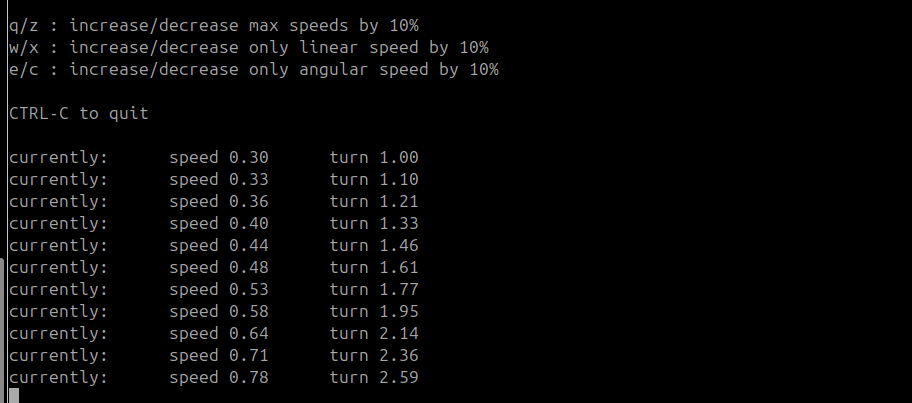
\includegraphics[width=0.94\textwidth]{teleop_2026-10-12_23-07-05.png}
\caption{Giao diện teleop và thao tác tăng giá trị đặt tốc độ; ảnh chụp ngày 12/10/2026.}
\label{fig:teleop}
\end{figure}

Để kiểm tra đường lệnh điều khiển, đọc \code{/cmd_vel} trong terminal khác khi
nhấn phím ở teleop:
\begin{lstlisting}
ros2 topic info /cmd_vel -v
ros2 topic echo /cmd_vel geometry_msgs/msg/TwistStamped \
  --qos-reliability best_effort
\end{lstlisting}

Phép kiểm tra ban đầu xác nhận subscriber chính là \code{motion_control}.
Một thử nghiệm tiến chậm trong world maze dùng cùng mô hình/controller cho
odometry thay đổi khoảng 0.045 m và kết thúc bằng lệnh vận tốc bằng 0.
Kết quả này chứng minh luồng vận tốc hoạt động trong phiên thử đó; không dùng
nó để kết luận robot đã đi hết world depot. Khi kiểm tra bài, cần đối chiếu
message vận tốc với chuyển động trong Gazebo và thay đổi của odometry,
vì chỉ có publisher trên \code{/cmd_vel} chưa đủ chứng minh robot nhận lệnh.

\subsection{TF và hiển thị RViz2}
Chuỗi TF rút gọn được minh họa ở Hình~\ref{fig:tf}. Biến đổi odom--base link
mô tả chuyển động của robot; các biến đổi tới LiDAR cho phép đặt dữ liệu scan
đúng vị trí. Scan dùng QoS Best Effort/Volatile trong cấu hình RViz của bài.
Khi chưa có bản đồ, fixed frame là odom; khi mapping hoặc localization,
fixed frame chuyển sang map.

\begin{figure}[htbp]
\centering
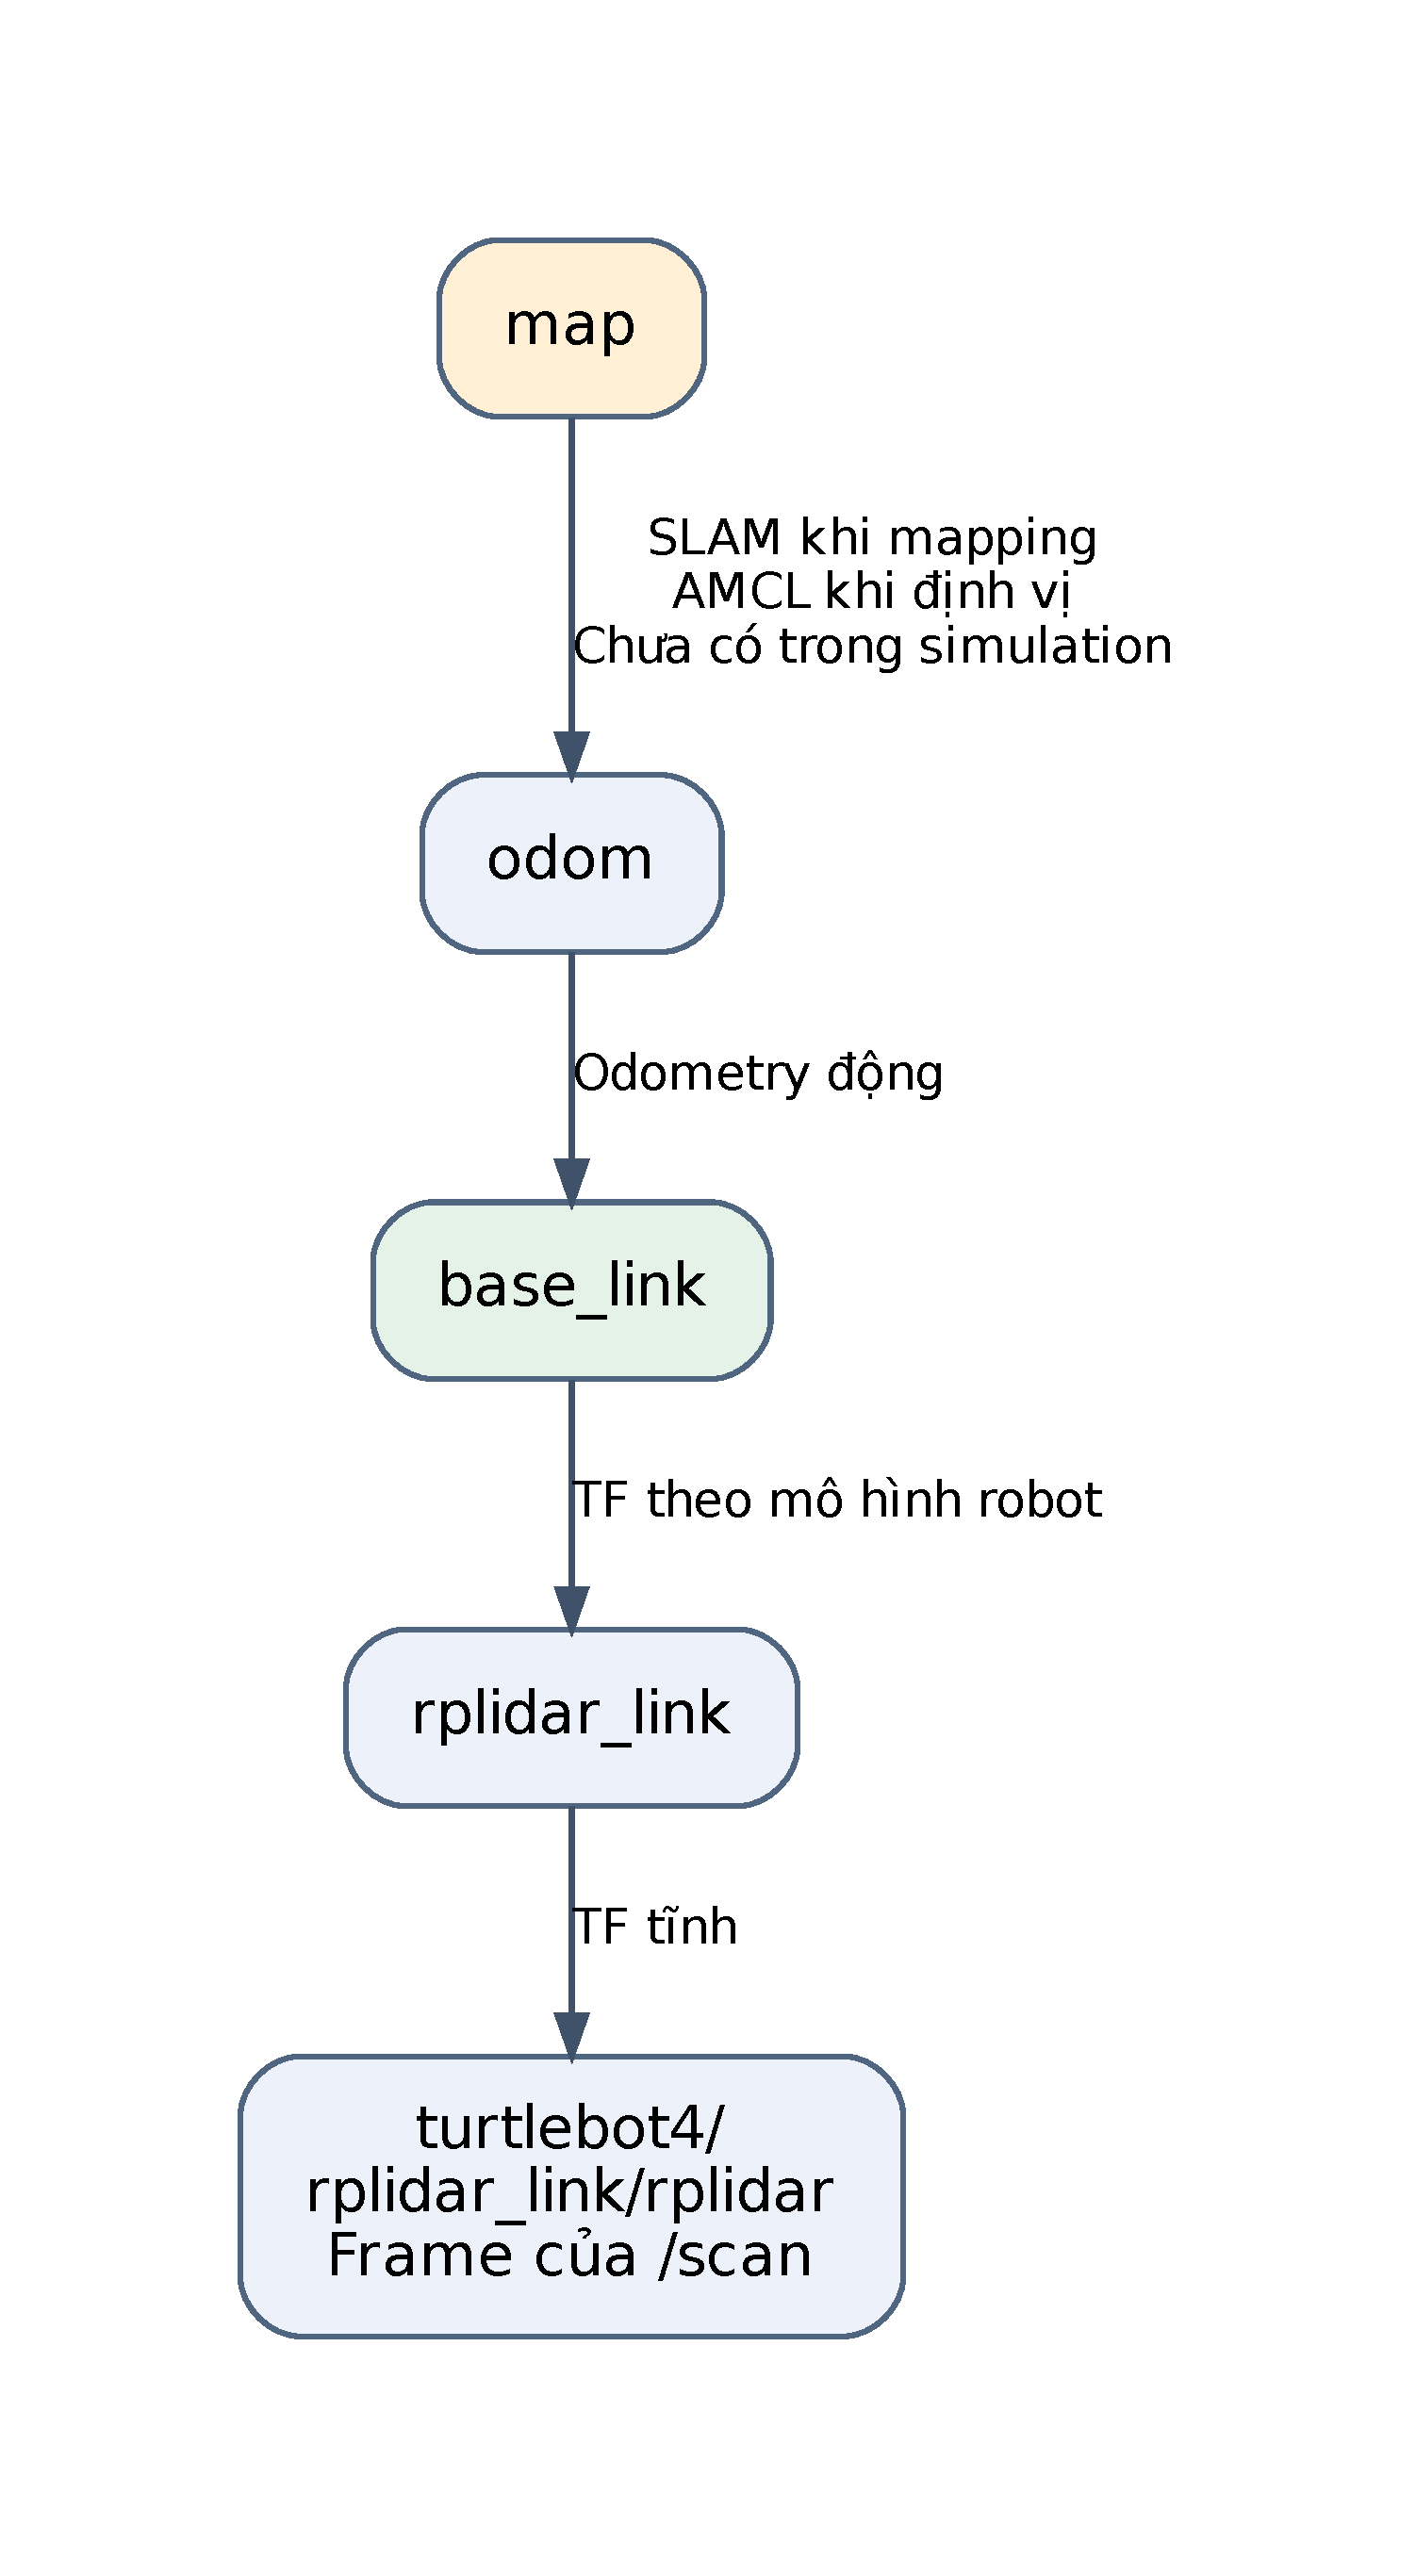
\includegraphics[width=0.74\textwidth,height=0.46\textheight,keepaspectratio]{02_tf.pdf}
\caption{Chuỗi TF rút gọn. Biến đổi map--odom do SLAM hoặc AMCL cung cấp theo chế độ.}
\label{fig:tf}
\end{figure}

\begin{lstlisting}
ros2 run tf2_ros tf2_echo odom base_link --ros-args \
  -p use_sim_time:=true
ros2 run tf2_ros tf2_echo base_link \
  turtlebot4/rplidar_link/rplidar --ros-args -p use_sim_time:=true
\end{lstlisting}
Các phép kiểm tra khi triển khai đã nhận được TF từ odom đến thân robot và
LiDAR. Bộ dữ liệu kiểm tra vì vậy có đủ điều kiện cho bước SLAM. Những ảnh
kiểm tra sensor/chuyển động trên depot cần được bổ sung vào bộ minh chứng
nghiệm thu để thể hiện đầy đủ Phần 1.

\FloatBarrier
\section{Xây dựng và lưu bản đồ bằng SLAM Toolbox}
\subsection{Nguyên lý và luồng dữ liệu}
SLAM giải quyết đồng thời việc ước lượng pose và dựng bản đồ khi chưa có map
môi trường. LiDAR cung cấp thông tin về tường, vật cản; TF odometry cung cấp
quan hệ chuyển động giữa các lần quét. Đối sánh scan ràng buộc các pose;
pose graph và loop closure hỗ trợ hiệu chỉnh khi robot quay lại khu vực đã đi.
SLAM Toolbox xuất occupancy map trên \code{/map} và TF map--odom
\cite{tb4mapping,slamtoolbox}.

Hình~\ref{fig:slam} phân biệt đầu ra phục vụ quan sát và bước lưu bản đồ.
Trong cấu hình sử dụng, đầu vào trực tiếp quan trọng của SLAM là scan và TF;
không đồng nhất việc kiểm tra topic odom với việc node SLAM phải subscribe
trực tiếp topic này.

\begin{figure}[htbp]
\centering
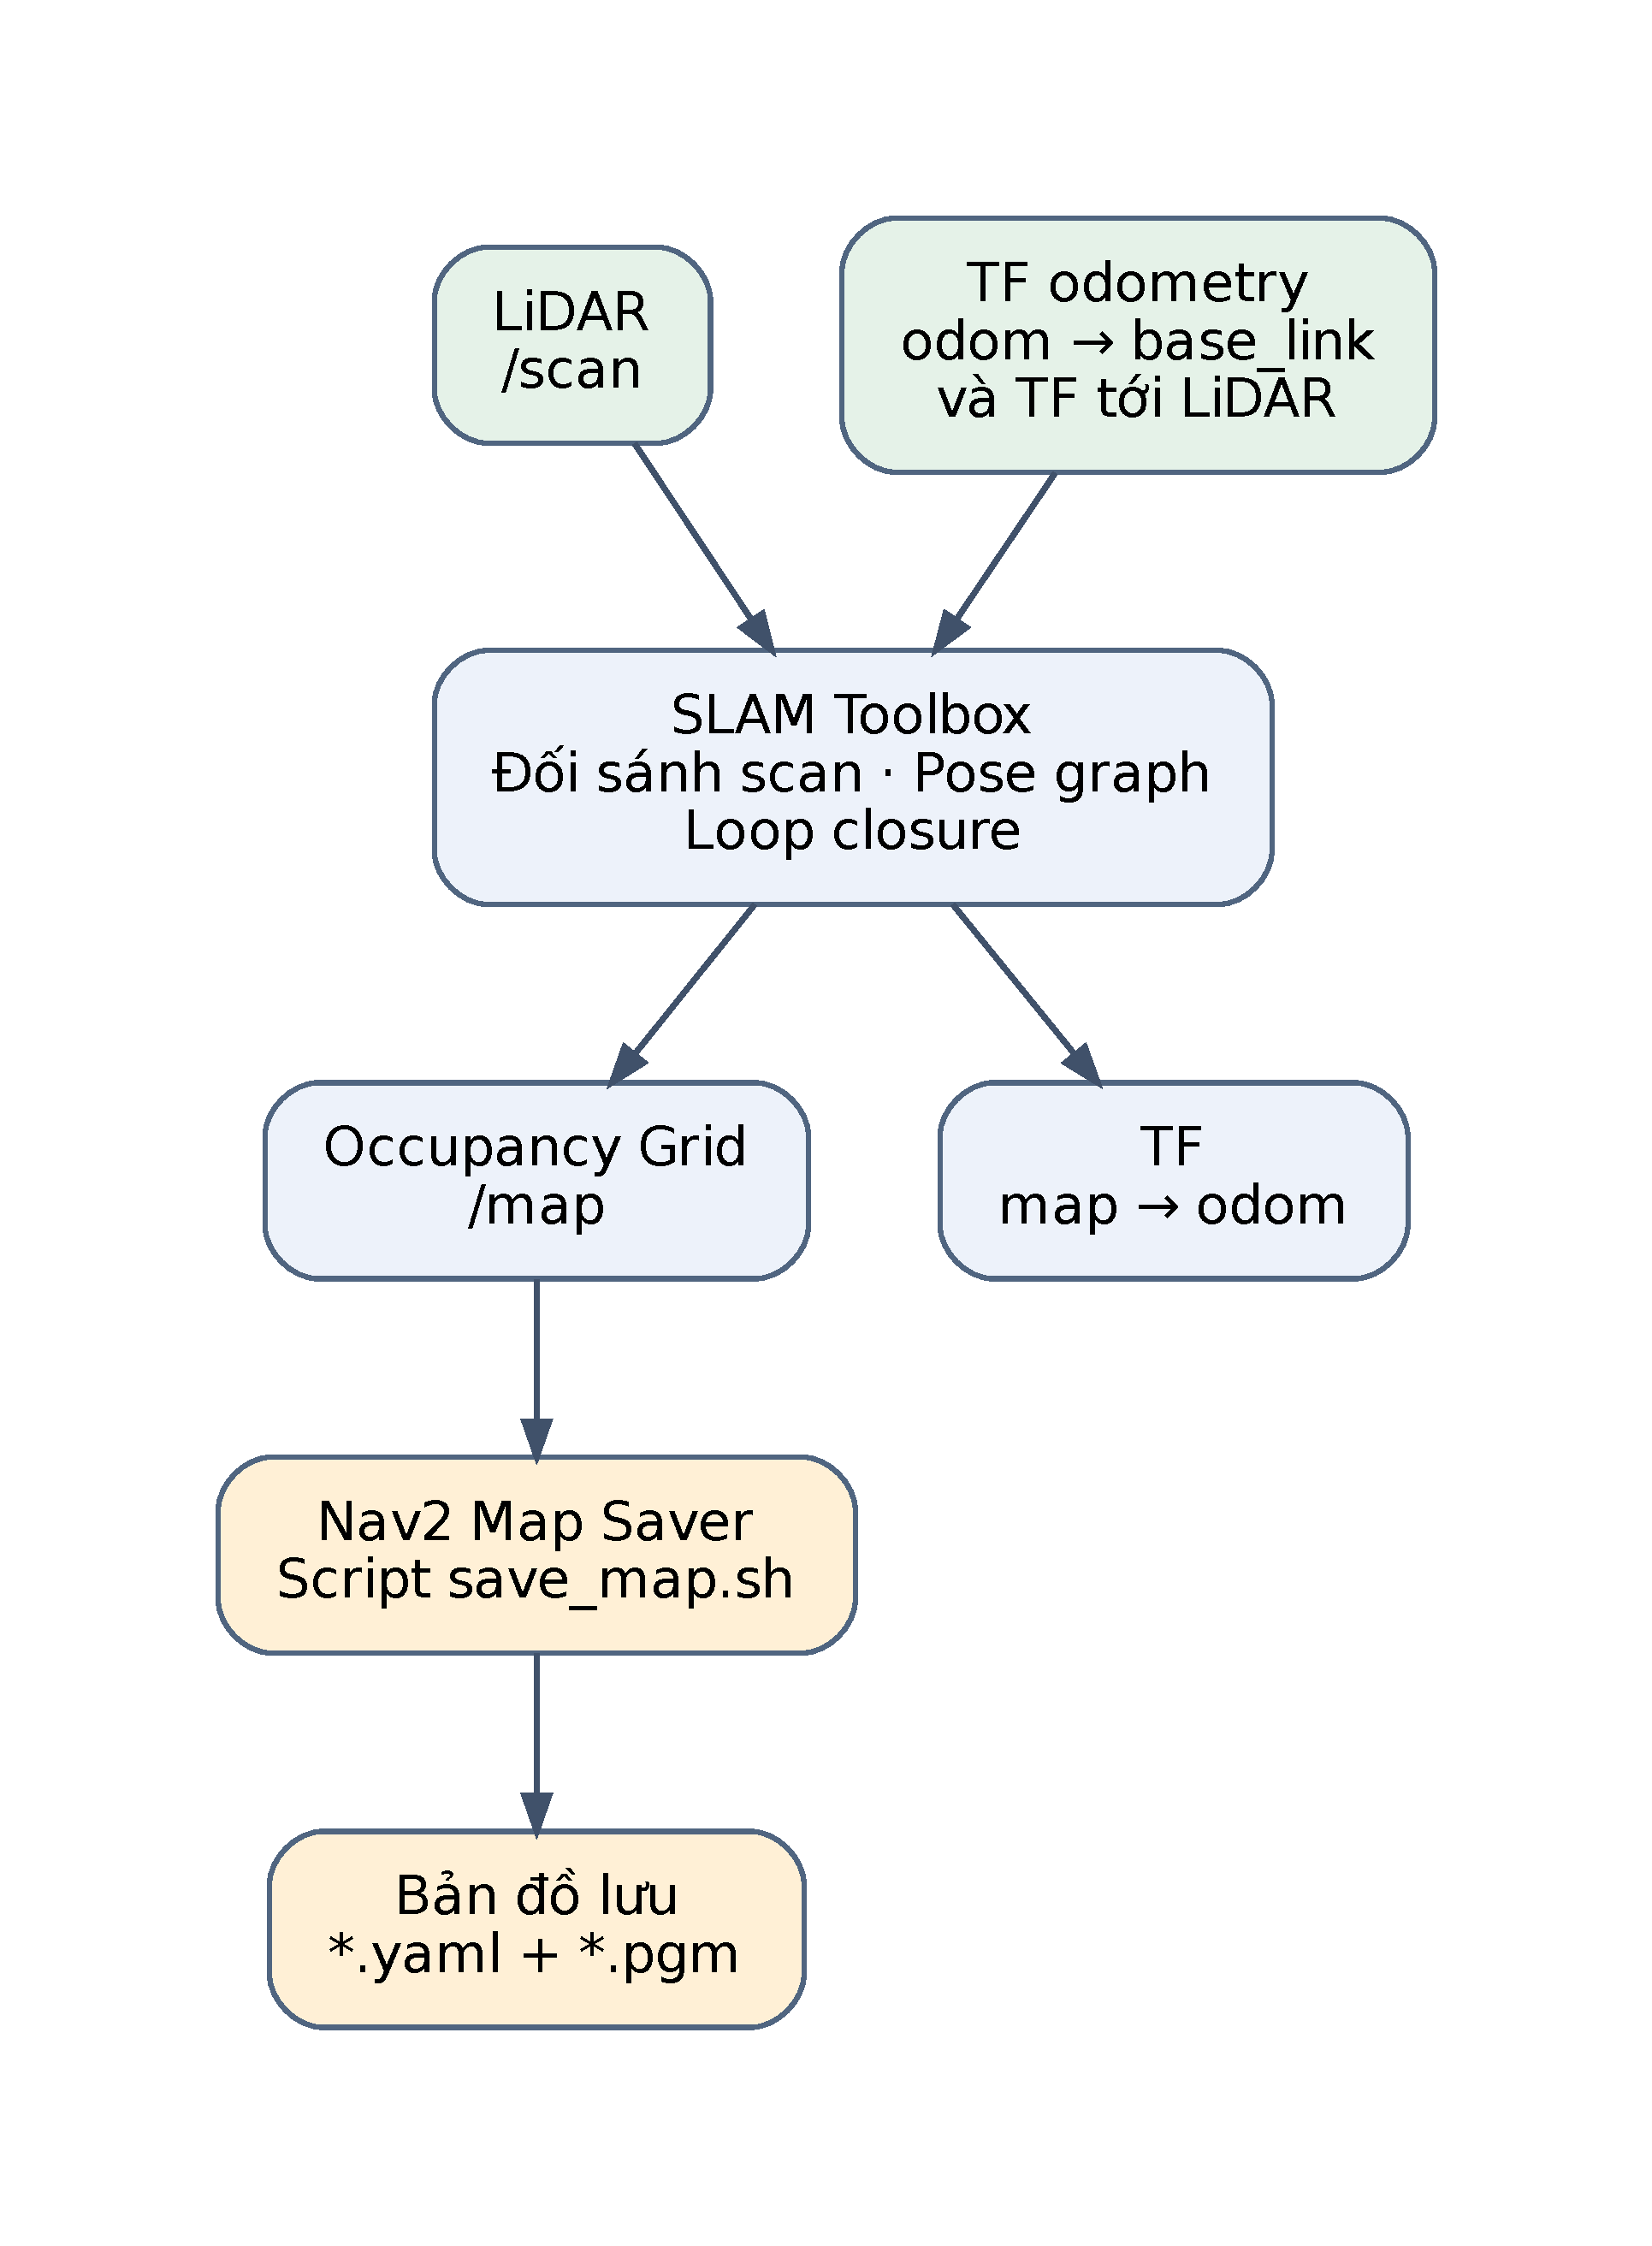
\includegraphics[width=0.75\textwidth,height=0.48\textheight,keepaspectratio]{03_slam.pdf}
\caption{Đầu vào, đầu ra và quá trình lưu bản đồ của SLAM Toolbox.}
\label{fig:slam}
\end{figure}

\subsection{Quy trình khảo sát}
Dừng teleop và launch simulation trước khi chuyển sang mapping:
\begin{lstlisting}
ros2 launch turtlebot4_slam_nav mapping.launch.py \
  world:=depot gui_render_engine:=ogre2
\end{lstlisting}
Launch này include SLAM Toolbox ở chế độ synchronous, giữ cấu hình chính thức
và chưa bật AMCL/Nav2. Robot mới cần được kiểm tra dock và undock trước khi
mở lại teleop. Trong quá trình khảo sát, quan sát bản đồ cập nhật trên RViz,
đi qua các lối đi và vùng quanh vật cản, quét những mặt khuất và trở lại vùng
quen thuộc để hỗ trợ đóng vòng. Ở lối hẹp cần giảm giá trị đặt tốc độ, hạn chế
đi sát vật cản hoặc quay quá nhanh. Đây là quy trình thực hiện; tỷ lệ bao phủ
cụ thể phải được đối chiếu bằng tuyến khảo sát và video.

Sau khi robot đứng yên, kiểm tra SLAM active và có map/TF:
\begin{lstlisting}
ros2 lifecycle get /slam_toolbox
ros2 topic echo /map nav_msgs/msg/OccupancyGrid \
  --once --field info --qos-durability transient_local
ros2 run tf2_ros tf2_echo map odom --ros-args -p use_sim_time:=true
\end{lstlisting}

\subsection{Lưu bản đồ và thông số thực nghiệm}
Script \code{save_map.sh} gọi Nav2 Map Saver để lưu occupancy map, tạo thư mục
đích nếu cần, kiểm tra mã thoát và kiểm tra đường dẫn ảnh trong YAML. Phải lưu
khi mapping còn chạy; chỉ dừng SLAM sau khi lưu thành công. Ví dụ:
\begin{lstlisting}
ros2 run turtlebot4_slam_nav save_map.sh \
  "$HOME/tb4_ws/src/turtlebot4_slam_nav/maps/depot_02"
\end{lstlisting}
Script không ghi đè file có sẵn. Nếu cần lưu một phiên khác, chọn tên mới thay
cho \code{depot_02}. Cặp file thực tế được cung cấp trong dự án có thông số
ở Bảng~\ref{tab:map}. PGM là ảnh lưới chiếm chỗ; YAML mô tả cách đọc ảnh,
độ phân giải, gốc tọa độ và các ngưỡng phân loại.

\begin{table}[htbp]
\centering\small
\caption{Thông số đọc từ bản đồ depot\_02 của dự án.}\label{tab:map}
\begin{tabularx}{\textwidth}{p{0.38\textwidth}Y}
\toprule
Thuộc tính & Giá trị \\
\midrule
YAML / ảnh tham chiếu & \code{depot_02.yaml} / \code{depot_02.pgm} \\
Kích thước ảnh & $602 \times 302$ ô \\
Resolution & $0.050$ m/ô \\
Origin $(x,y,\theta)$ & $(-15.117, -7.709, 0)$ \\
Mode / negate & \code{trinary} / $0$ \\
Free / occupied threshold & $0.196$ / $0.65$ \\
Kích thước lưới theo mét & $30.10 \times 15.10$ m \\
\bottomrule
\end{tabularx}
\end{table}

Kích thước theo mét là kích thước toàn lưới từ số ô và resolution, không phải
chiều dài tuyến khảo sát hoặc diện tích đã được robot khám phá. Bản đồ được
biểu diễn trực tiếp từ file PGM trong Hình~\ref{fig:map}; không sử dụng bản đồ
mẫu của package thay cho sản phẩm thực nghiệm.

\begin{figure}[htbp]
\centering
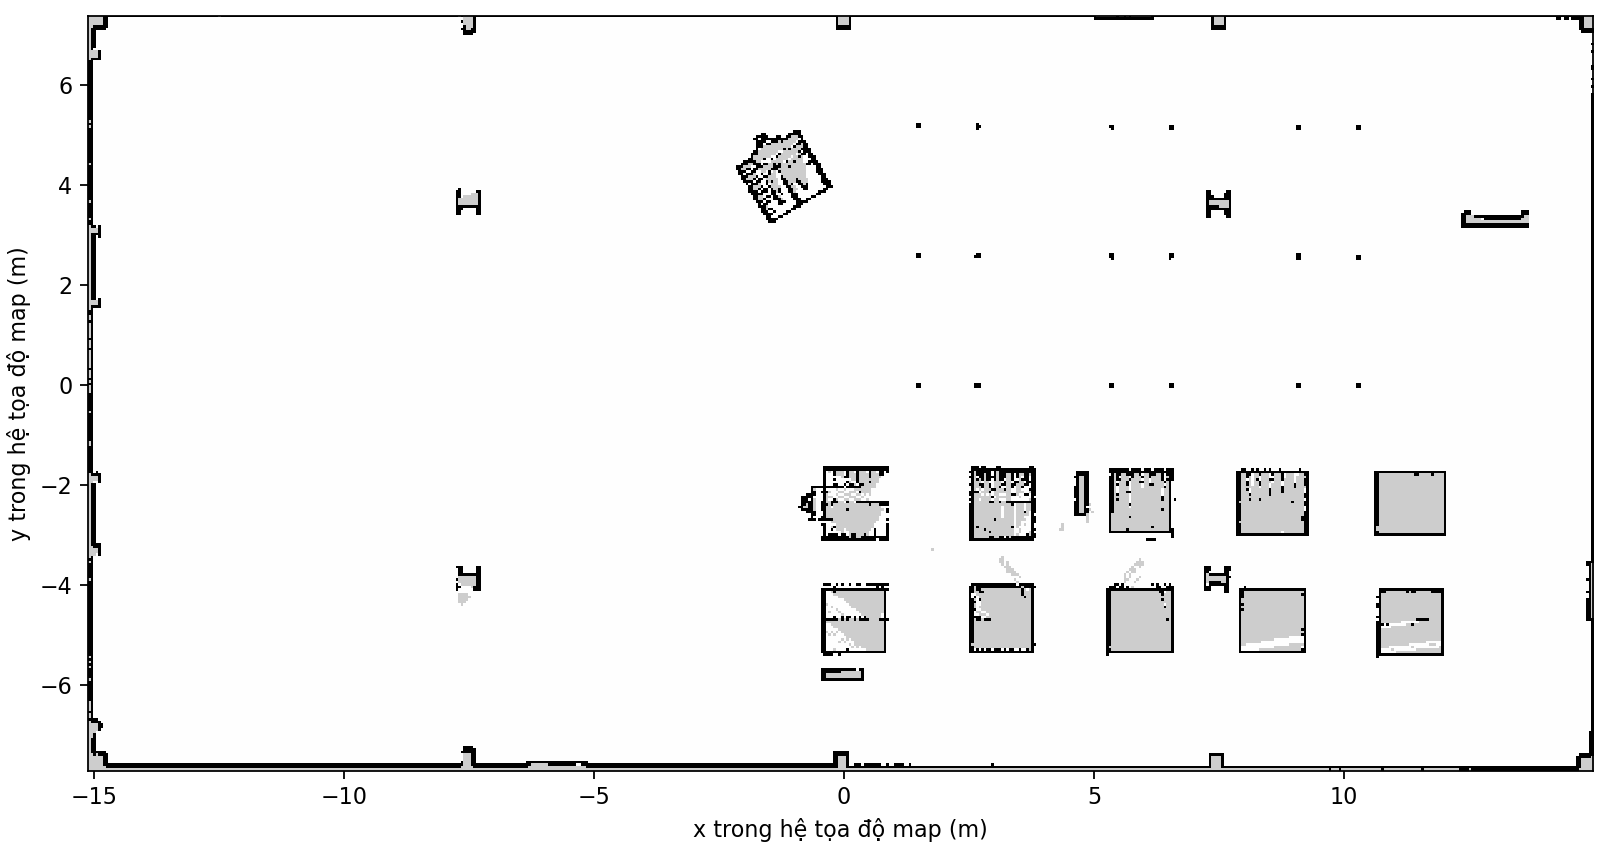
\includegraphics[width=\textwidth]{depot_02_map.png}
\caption{Bản đồ occupancy depot\_02 đọc từ PGM thật, với trục tọa độ map theo thông số YAML.}
\label{fig:map}
\end{figure}

Quan sát ảnh cho phép nhận diện biên ngoài và các cụm vật cản bên trong.
Các vùng quanh một số vật cản có biên không hoàn toàn đều, cần kiểm tra thêm
bằng đối chiếu world và dữ liệu khảo sát. Tường phải rõ, hành lang liên tục và
không có các lớp tường bị nhân đôi rõ rệt. Bộ minh chứng hiện tại chưa có
chuỗi ảnh/video khảo sát để định lượng mức độ bao phủ; vì vậy không kết luận
đã khảo sát phần lớn môi trường chỉ dựa vào kích thước ảnh map.

\FloatBarrier
\section{Localization trên bản đồ đã lưu}
\subsection{Nạp map và khởi tạo pose}
Sau khi lưu map, dừng SLAM rồi khởi động lại cùng world, model và pose spawn.
Chế độ localization nạp map server và AMCL, chưa chạy Nav2:
\begin{lstlisting}
ros2 launch turtlebot4_slam_nav localization.launch.py \
  world:=depot gui_render_engine:=ogre2 \
  map:="$HOME/tb4_ws/src/turtlebot4_slam_nav/maps/depot_02.yaml"
\end{lstlisting}

Map server xuất bản map tĩnh. AMCL sử dụng bản đồ, scan và thông tin chuyển
động để ước lượng pose bằng bộ lọc hạt; đầu ra gồm pose và TF map--odom.
Trên RViz, công cụ \textbf{2D Pose Estimate} cung cấp ước lượng ban đầu
\cite{tb4navigation}. Nhấn tại vị trí hiện tại của robot trên bản đồ và kéo
mũi tên theo hướng robot. Sau undock, robot đã rời vị trí spawn; tọa độ map
cũng không nhất thiết trùng tọa độ world Gazebo.
Hình~\ref{fig:amcl} tóm tắt các đầu vào và đầu ra của định vị.

\begin{figure}[htbp]
\centering
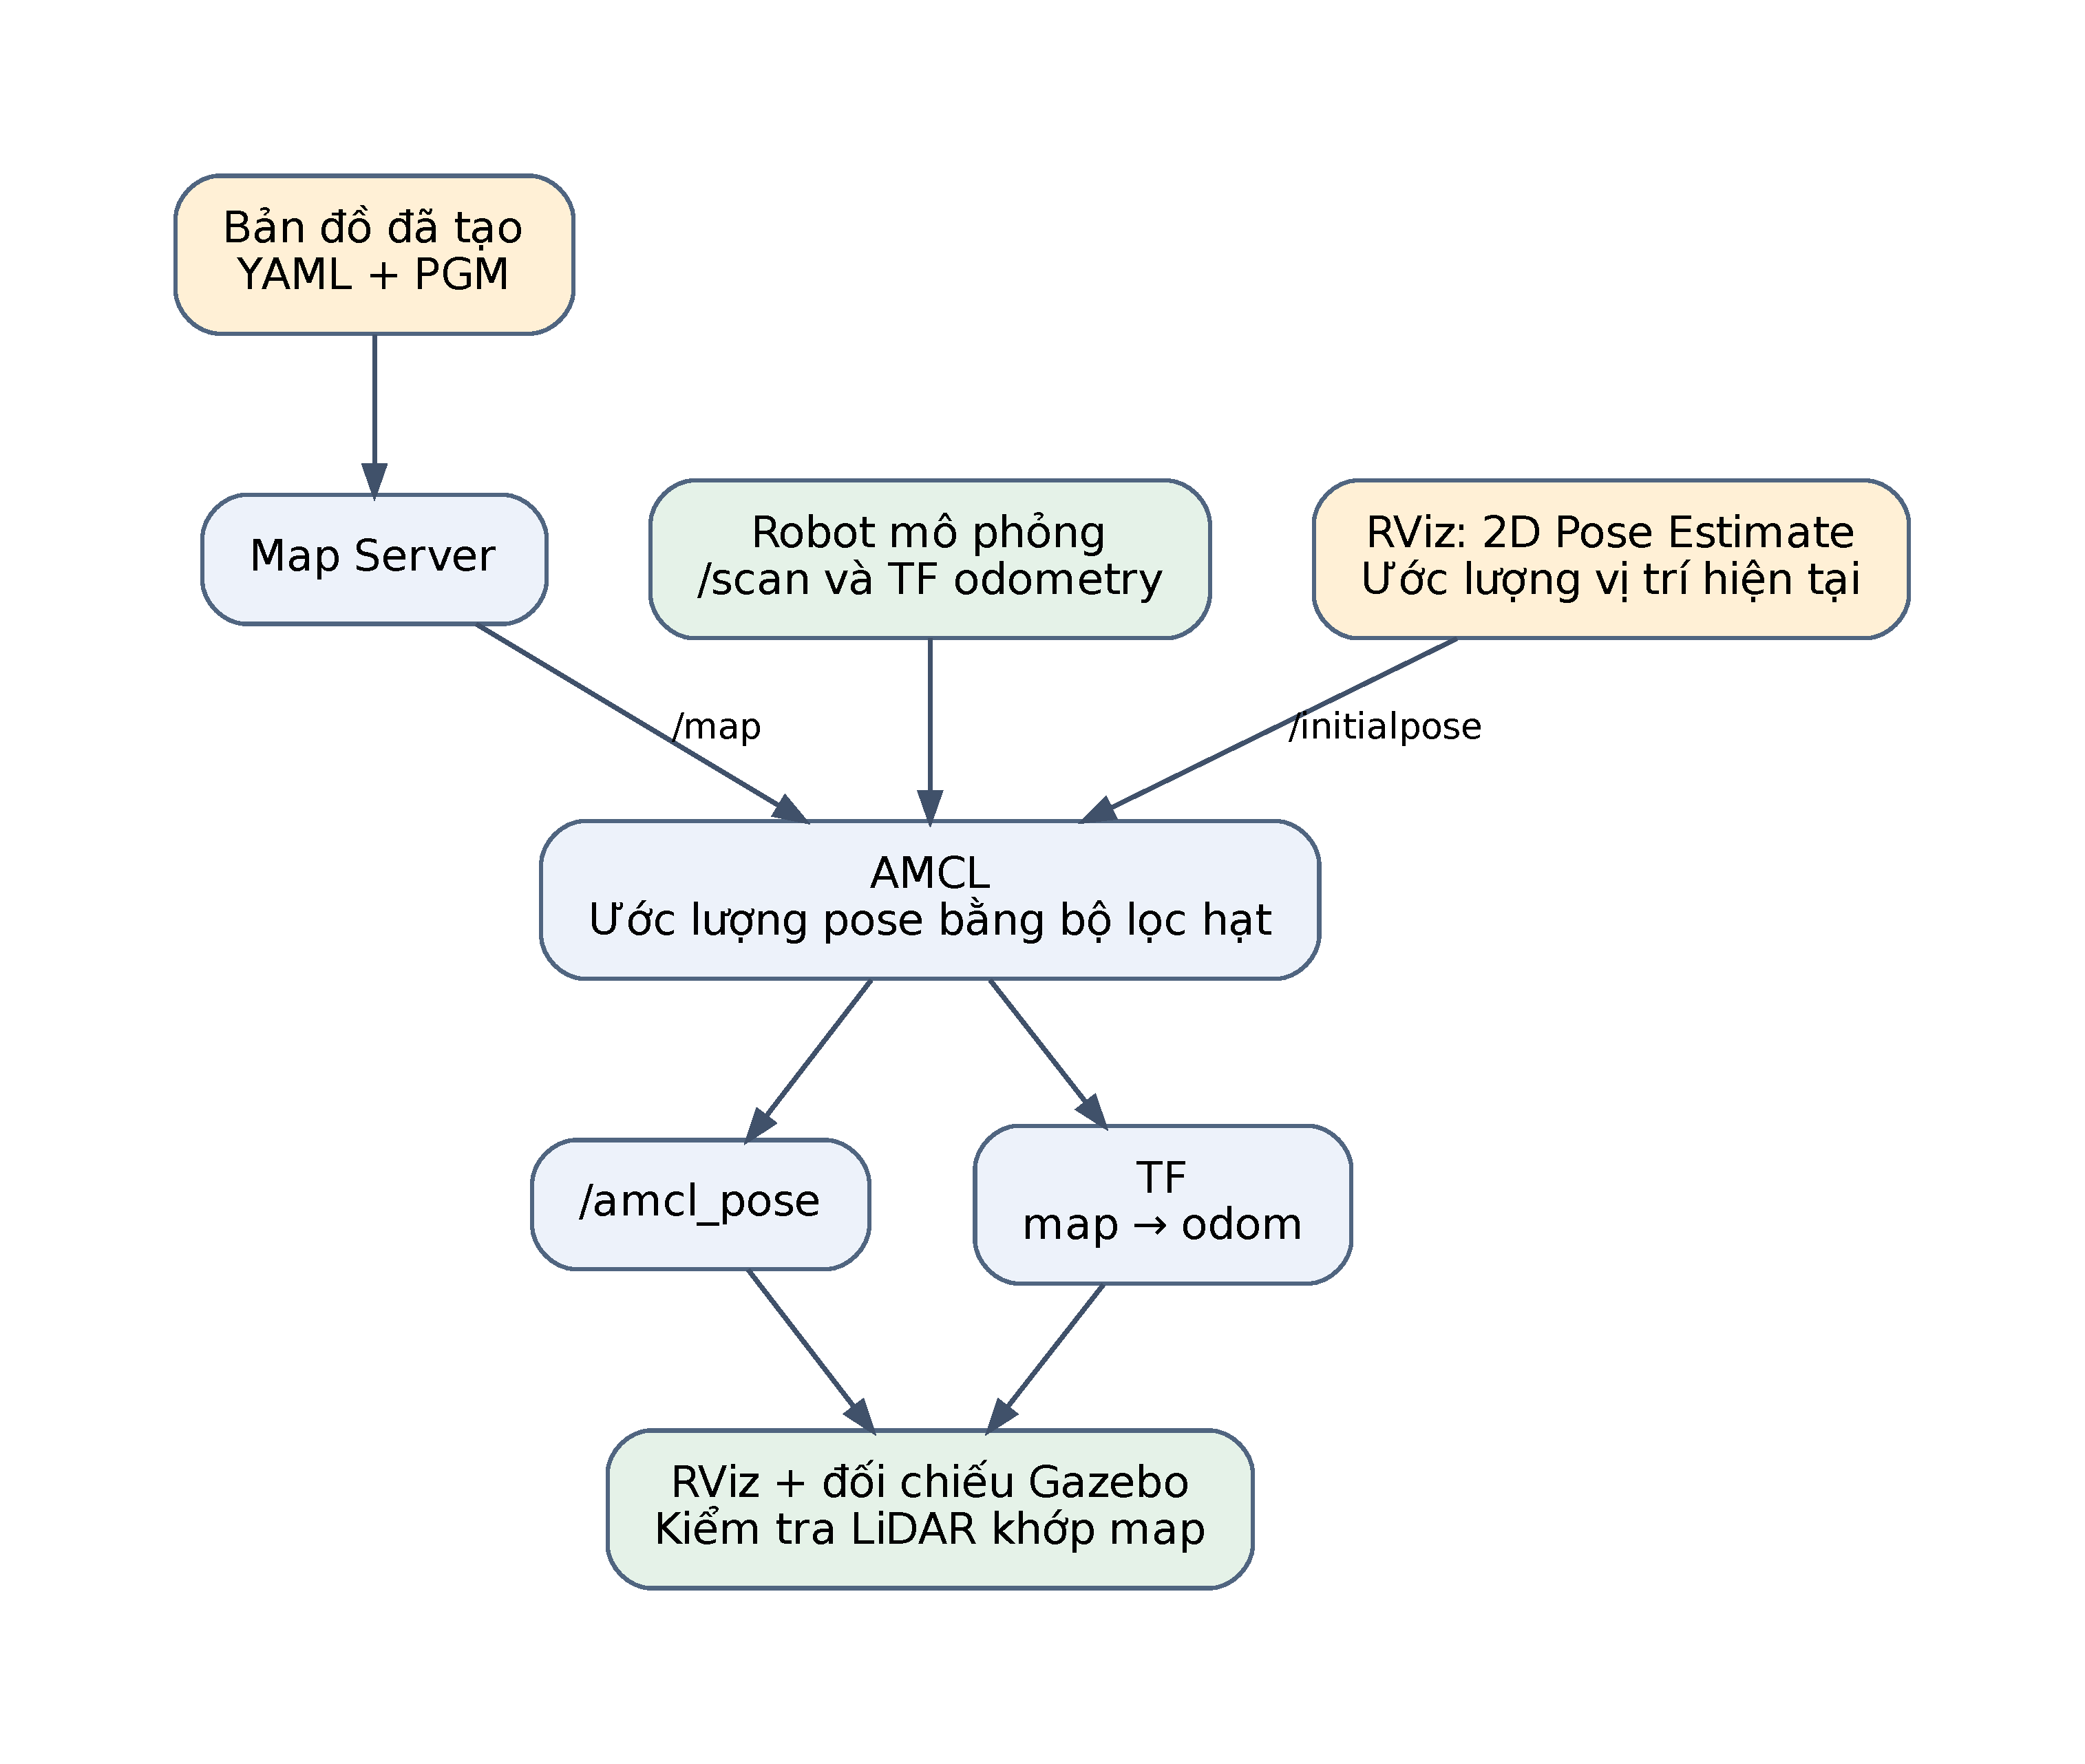
\includegraphics[width=0.88\textwidth,height=0.48\textheight,keepaspectratio]{04_localization.pdf}
\caption{Luồng định vị bằng map server và AMCL trên bản đồ đã lưu.}
\label{fig:amcl}
\end{figure}

\subsection{Kiểm tra và kết quả quan sát}
Các lệnh kiểm tra gồm trạng thái lifecycle, pose và TF:
\begin{lstlisting}
ros2 lifecycle get /map_server
ros2 lifecycle get /amcl
ros2 topic echo /amcl_pose geometry_msgs/msg/PoseWithCovarianceStamped --once
ros2 run tf2_ros tf2_echo map base_link --ros-args -p use_sim_time:=true
\end{lstlisting}

Log do người thực hiện cung cấp ghi nhận AMCL nhận initial pose và tiếp tục
\code{Setting pose}. Hai lần đặt pose có cảnh báo extrapolation vào tương lai
khoảng 6 ms và 18 ms so với TF odometry mới nhất. AMCL vẫn xử lý pose sau
cảnh báo này; việc nhận pose chưa tự chứng minh vị trí đã chính xác.
Cần xác nhận pose được xuất bản, chuỗi map--odom--base link có dữ liệu và scan
chồng lên biên tường/vật cản. Trước initial pose, thiếu TF từ map có thể làm
RViz giữ scan rồi bỏ message khi queue đầy.

Ảnh thực nghiệm ở Hình~\ref{fig:localization} cho thấy RViz ở chế độ localization,
Map, RobotModel, LaserScan và tập hạt AMCL được bật; Global Status là Ok.
Một số điểm LiDAR nằm gần biên các vật cản trên map. Tuy nhiên, chưa có ảnh
Gazebo cùng trạng thái để đối chiếu trực tiếp vị trí và hướng robot, nên mức
độ khớp pose cần được bổ sung trong minh chứng nghiệm thu.

\begin{figure}[htbp]
\centering
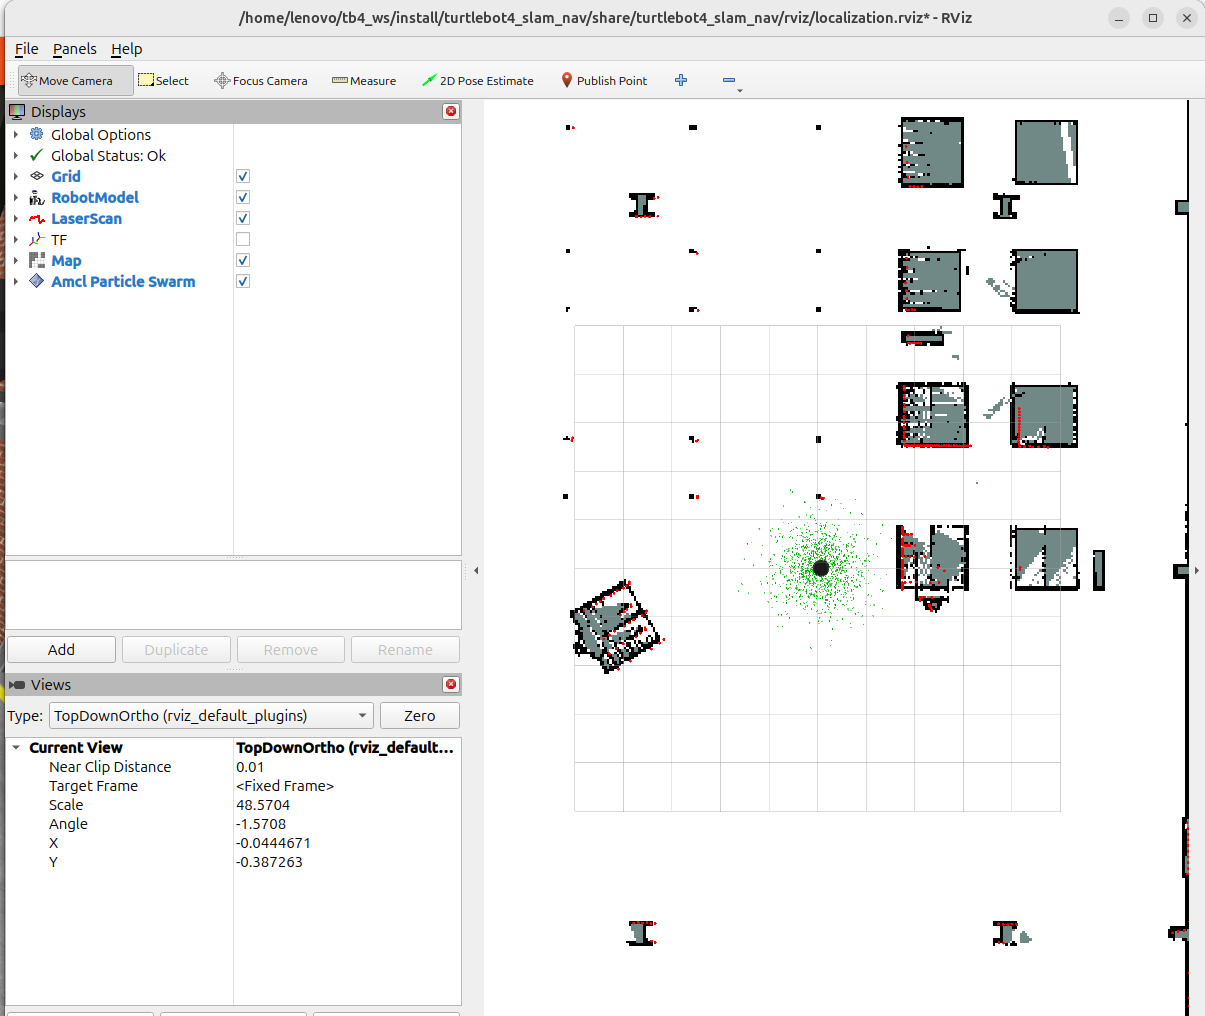
\includegraphics[width=0.84\textwidth,height=0.58\textheight,keepaspectratio]{localization_rviz_2026-10-12_23-30-06.png}
\caption{RViz localization lúc 23:30:06 ngày 12/10/2026: bản đồ, robot, LiDAR và tập hạt AMCL.}
\label{fig:localization}
\end{figure}

\FloatBarrier
\section{Điều hướng tự động bằng Nav2}
\subsection{Khởi chạy và luồng xử lý goal}
Sau khi kiểm tra localization, dừng phiên cũ và chạy navigation. Chế độ này
include map server, AMCL và Nav2, không chạy SLAM:
\begin{lstlisting}
ros2 launch turtlebot4_slam_nav navigation.launch.py \
  world:=depot gui_render_engine:=ogre2 \
  map:="$HOME/tb4_ws/src/turtlebot4_slam_nav/maps/depot_02.yaml"
ros2 lifecycle get /controller_server
ros2 lifecycle get /bt_navigator
ros2 lifecycle get /collision_monitor
ros2 action info /navigate_to_pose
\end{lstlisting}

Robot mới cần undock và đặt initial pose. Sau khi LiDAR khớp map và Nav2 active,
thoát teleop trước khi gửi goal. Cần phân biệt \textbf{2D Pose Estimate} là
ước lượng vị trí hiện tại, còn \textbf{Nav2 Goal} là đích robot phải tự đi tới.
Chỉ chạy localization sẽ không có hệ thống điều hướng để thực hiện goal.

BT navigator quản lý tiến trình hành vi. Planner server tính đường đi toàn
cục theo costmap; controller server dùng path, trạng thái robot và local
costmap để tính lệnh vận tốc. Trong cấu hình chính thức đang dùng, lệnh đi
qua velocity smoother và collision monitor trước khi tới motion control,
controller bánh xe và Gazebo bridge. Luồng này được minh họa ở
Hình~\ref{fig:navflow}; sơ đồ giản lược các nhánh hành vi phụ để tập trung vào
navigation tới một pose \cite{nav2}.

\begin{figure}[htbp]
\centering
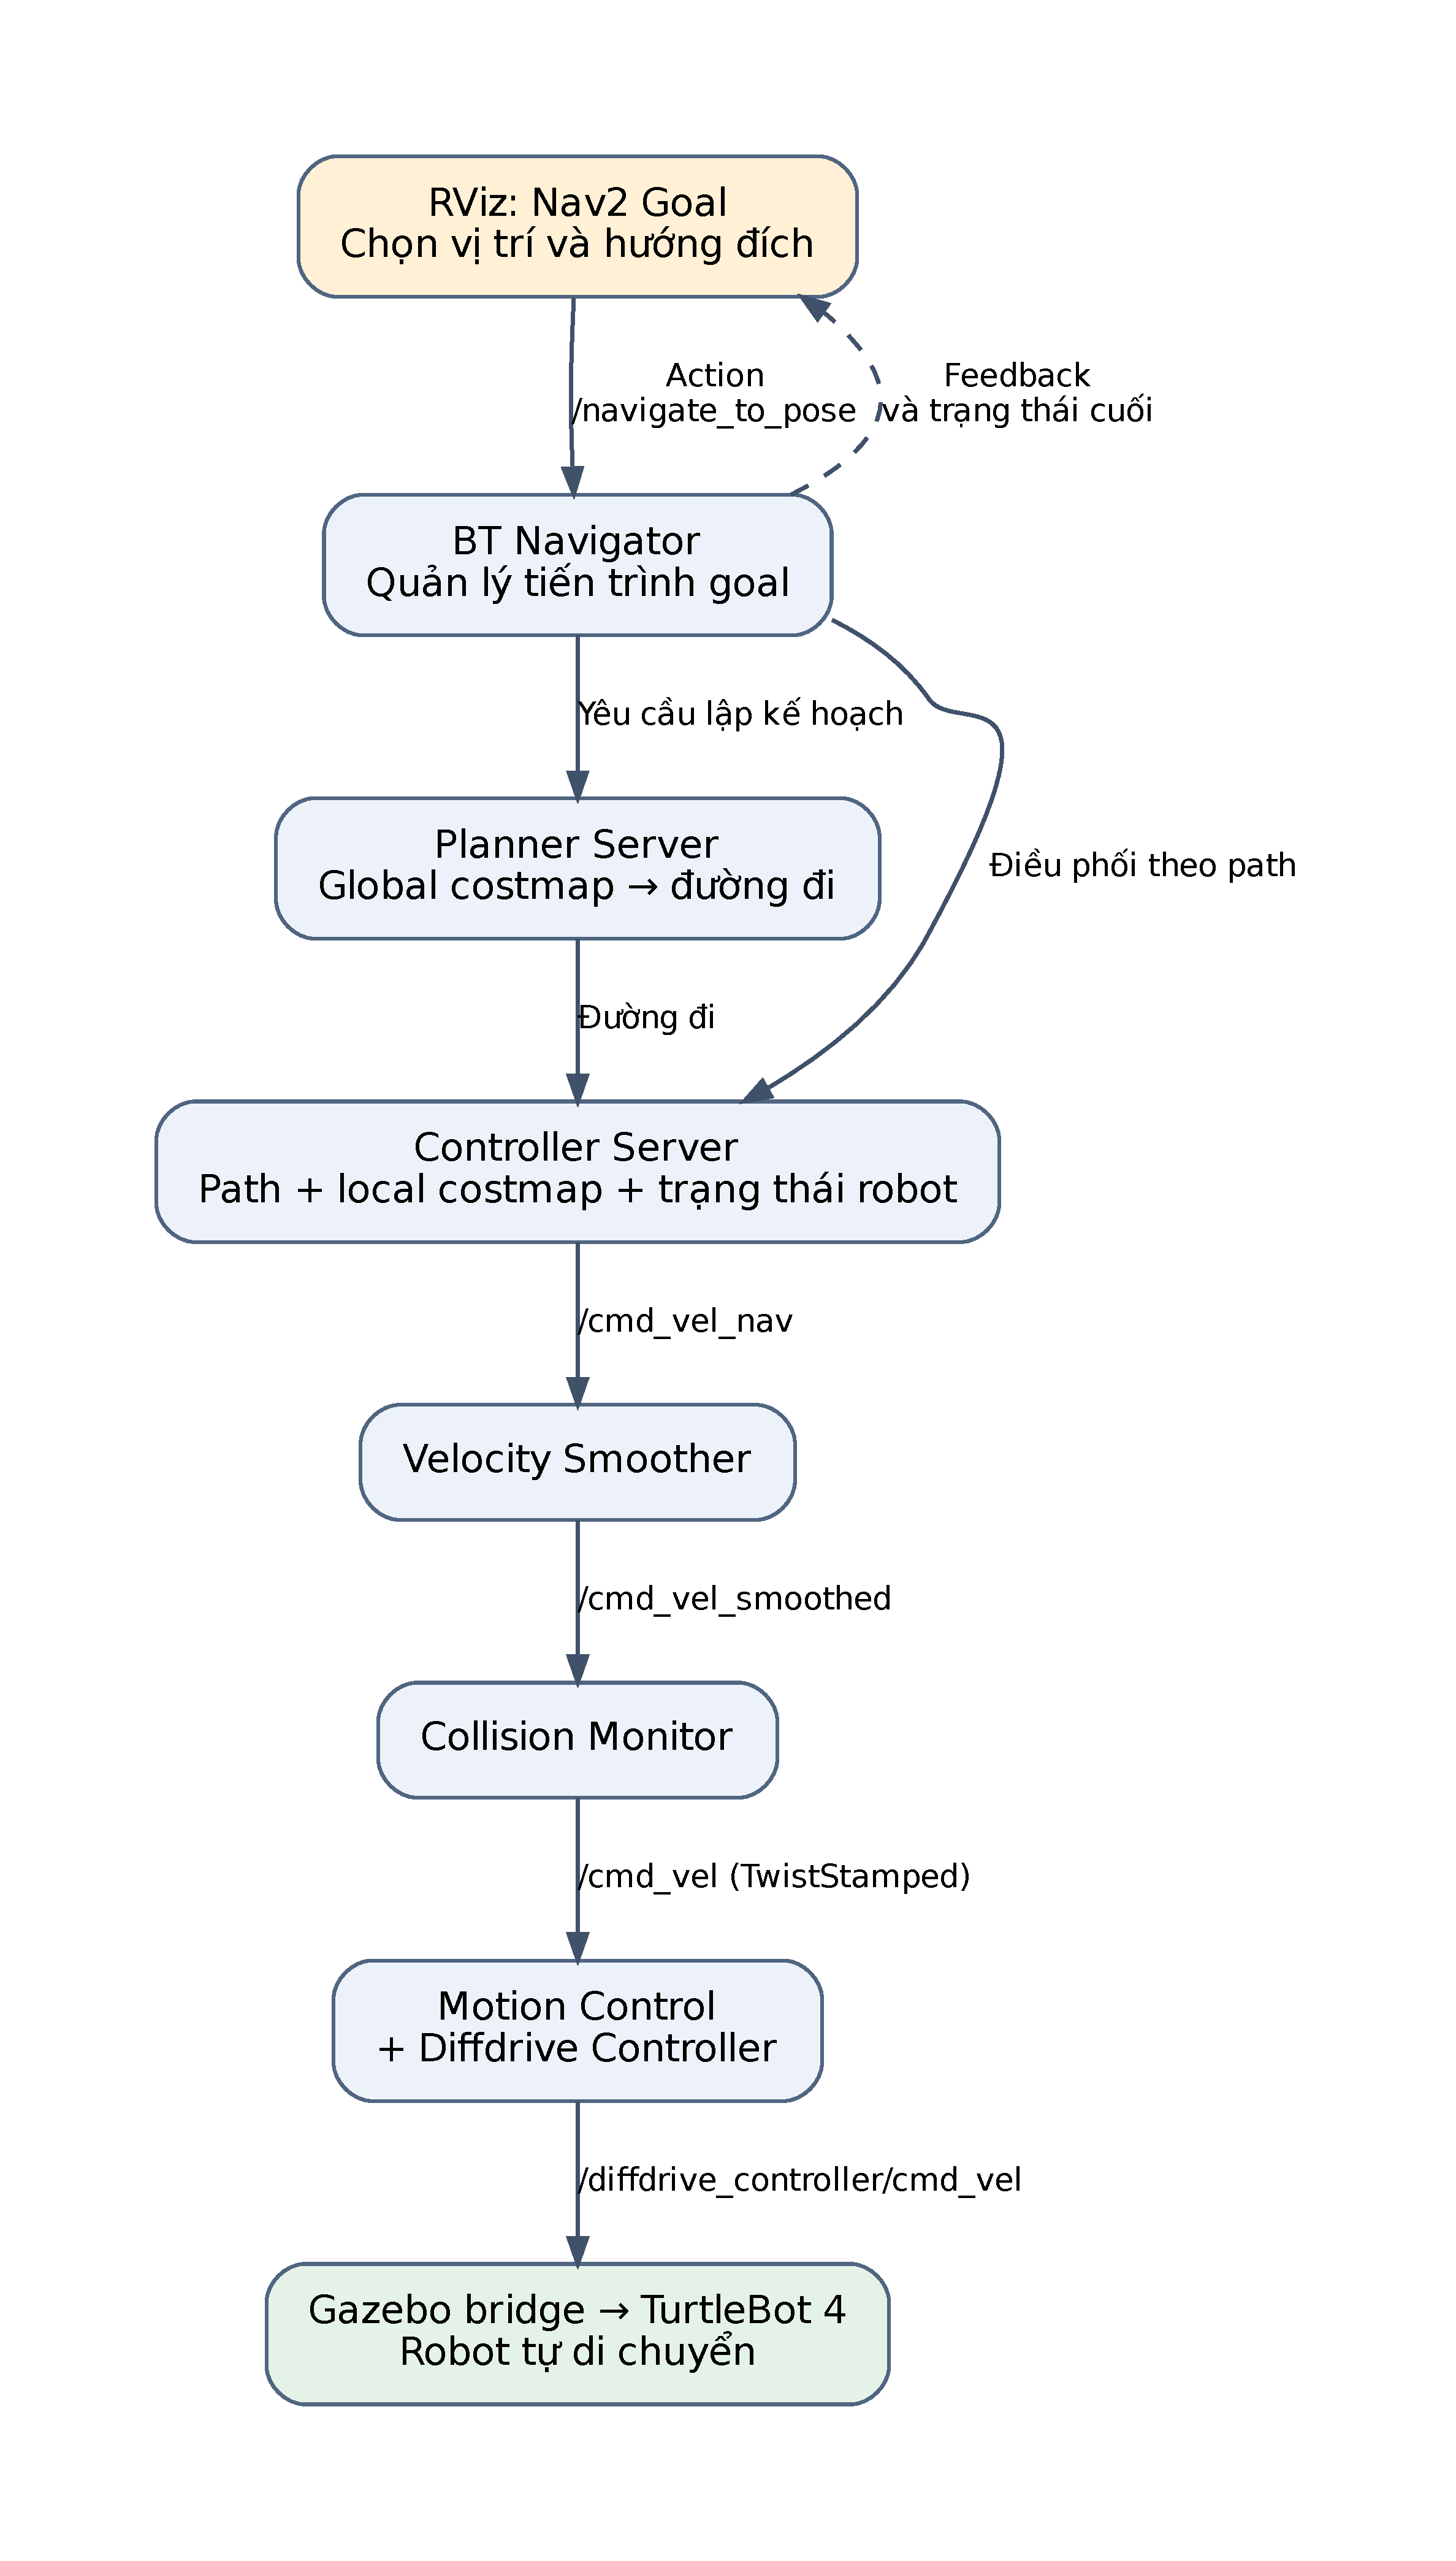
\includegraphics[width=0.84\textwidth,height=0.60\textheight,keepaspectratio]{05_navigation.pdf}
\caption{Luồng goal, lập kế hoạch và xử lý lệnh vận tốc của Nav2.}
\label{fig:navflow}
\end{figure}

\subsection{Quy trình ba goal và theo dõi trạng thái}
Chọn ba mục tiêu trong vùng trống đã được map, ở các khu vực khác nhau và có
khoảng cách phù hợp tới vật cản. Trên RViz, dùng Nav2 Goal, nhấn vị trí đích
và kéo mũi tên theo hướng mong muốn. Sau mỗi lần gửi, chờ robot tới đích và
trạng thái cuối thành công rồi mới gửi goal tiếp theo. Không điều khiển robot
thủ công sau khi gửi goal. Nếu localization vẫn đúng, không cần đặt lại
initial pose trước mỗi goal.

Theo dõi trạng thái action bằng:
\begin{lstlisting}
ros2 topic echo /navigate_to_pose/_action/status \
  action_msgs/msg/GoalStatusArray
\end{lstlisting}

Trạng thái \code{SUCCEEDED} có giá trị 4; \code{ABORTED} có giá trị 6 và không
được tính là thành công. Khi status chứa nhiều goal, phải đối chiếu đúng UUID,
không lấy kết quả của goal cũ cho goal mới. Để xác nhận không va chạm và không
có can thiệp thủ công, cần xem quá trình di chuyển qua video hoặc quan sát liên tục.

\subsection{Kết quả thực nghiệm hiện có}
Hình~\ref{fig:navresult} là ảnh được cung cấp ở thời điểm 23:35:20 ngày
12/10/2026. Navigation 2 panel hiển thị Navigation và Localization active,
Feedback là reached và Recoveries là 0. Ảnh này là minh chứng trực quan cho
một lần goal có phản hồi reached. Nó chưa xác định thứ tự/UUID của goal và
không thay thế video toàn bộ quá trình điều hướng.

\begin{figure}[htbp]
\centering
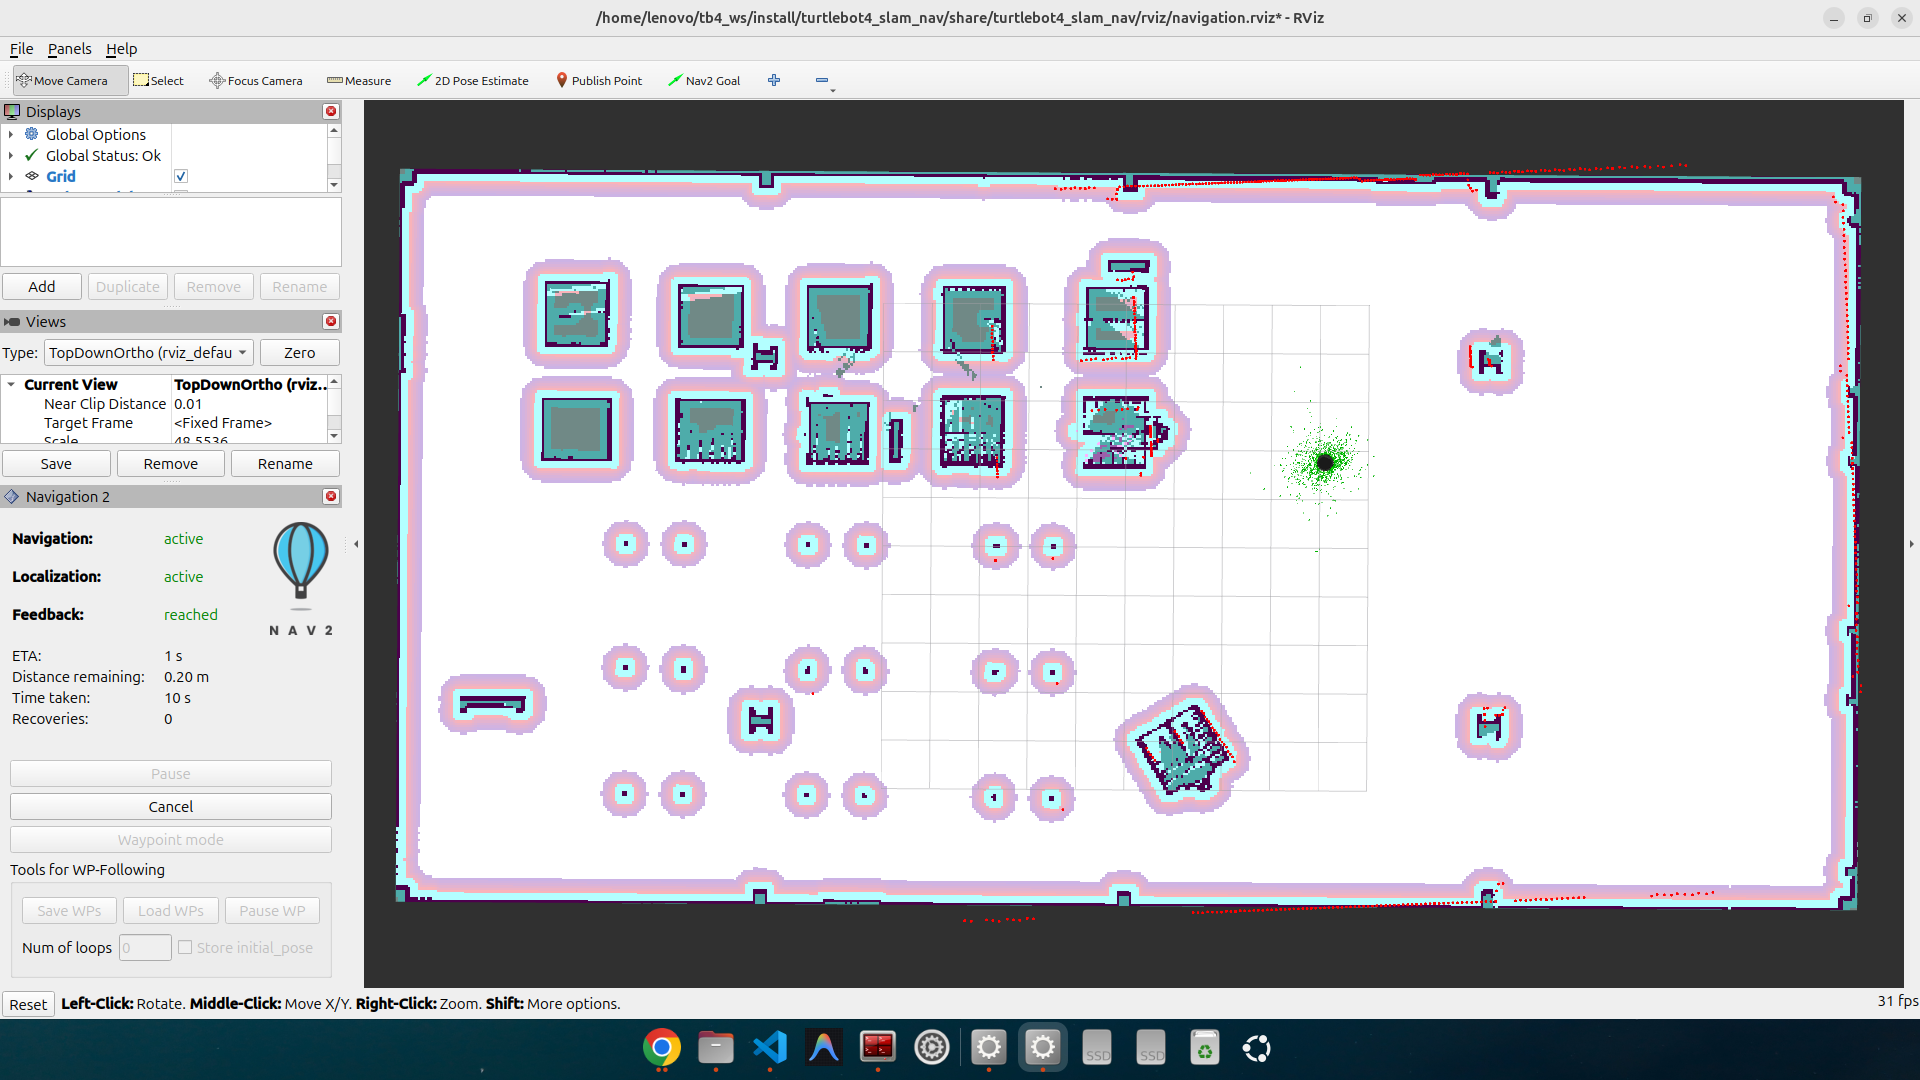
\includegraphics[width=\textwidth]{navigation_reached_2026-10-12_23-35-20.png}
\caption{Giao diện Nav2 hiển thị Navigation/Localization active và Feedback reached sau một goal.}
\label{fig:navresult}
\end{figure}

\begin{table}[htbp]
\centering\small
\caption{Đối chiếu bộ minh chứng hiện có với yêu cầu ba goal.}\label{tab:goals}
\begin{tabularx}{\textwidth}{p{0.21\textwidth}Y Y}
\toprule
Minh chứng & Kết quả quan sát được & Nội dung cần bổ sung \\
\midrule
Goal có ảnh lúc 23:35:20 & Navigation/Localization active; Feedback reached; Recoveries 0. & Số thứ tự, tọa độ/hướng goal, UUID hoặc mốc video. \\
Goal tại khu vực khác thứ nhất & Chưa có ảnh/log kèm theo bộ minh chứng. & Vị trí đích và trạng thái cuối đúng goal. \\
Goal tại khu vực khác thứ hai & Chưa có ảnh/log kèm theo bộ minh chứng. & Vị trí đích và trạng thái cuối đúng goal. \\
\bottomrule
\end{tabularx}
\end{table}

Bảng~\ref{tab:goals} phản ánh giới hạn của tài liệu được cung cấp, không khẳng
định hai goal còn lại chưa từng được thực hiện. Trước khi nộp báo cáo, cần bổ
sung ảnh/log hoặc video để xác nhận ba mục tiêu khác nhau đều thành công.
Các giá trị ETA, distance remaining và time taken trên panel là số hiển thị
tại thời điểm chụp; không dùng riêng ảnh này để đo thời gian thực của cả thí nghiệm.

\FloatBarrier
\section{Kết quả tổng hợp, vấn đề gặp phải và kết luận}
\subsection{Kết quả đã kiểm chứng}
Các kiểm tra mã nguồn khi triển khai gồm cú pháp Python/shell, dependency,
build package và đọc launch arguments của cả bốn chế độ. Build thành công;
bộ test có 7 mục, 6 mục chạy thành công và 1 test copyright có sẵn được skip.
Các phép kiểm tra mô phỏng đã nhận clock, scan, odometry, TF và xác nhận luồng
TwistStamped. Bản đồ depot\_02 tồn tại dưới dạng YAML/PGM và đã được đọc trực
tiếp để tạo hình bản đồ trong báo cáo.

Bộ ảnh người thực hiện cung cấp bổ sung bằng chứng về teleop, hiển thị
localization và một goal có Feedback reached. Mức độ hoàn thành được tổng
hợp trong Bảng~\ref{tab:results}; trạng thái node active không được đồng nhất
với việc hoàn thành toàn bộ yêu cầu khảo sát và ba navigation goal.

\begin{table}[htbp]
\centering\small
\caption{Tổng hợp kết quả và giới hạn của bộ minh chứng.}\label{tab:results}
\begin{tabularx}{\textwidth}{p{0.31\textwidth}Y}
\toprule
Yêu cầu & Kết quả/giới hạn hiện có \\
\midrule
Mô phỏng và topic cơ bản & Đã kiểm tra clock, scan, odometry, TF và chuyển động ở phiên triển khai; cần bổ sung ảnh Gazebo và topic của phiên nghiệm thu. \\
Teleoperation & Có ảnh giao diện và giá trị đặt tốc độ; kiểm tra luồng TwistStamped đã được thực hiện. \\
Bản đồ YAML/PGM & Có cặp depot\_02 thật, kích thước 602 × 302 ô, resolution 0.05 m/ô. \\
Bao phủ/chất lượng map & Có ảnh map để đánh giá hình học; chưa định lượng tỷ lệ khảo sát hoặc đối chiếu đầy đủ world. \\
Localization & Có ảnh RViz với map, LiDAR và tập hạt; các phiên kiểm tra đã có AMCL pose/TF. Cần ảnh đối chiếu Gazebo cùng trạng thái. \\
Navigation & Có ảnh một goal reached; cần bổ sung hai goal khác và video kiểm chứng không va chạm/can thiệp thủ công. \\
\bottomrule
\end{tabularx}
\end{table}

\subsection{Các vấn đề gặp phải và cách xử lý}
\paragraph{GUI Gazebo và môi trường terminal.}
Ban đầu các biến GUI kế thừa từ VS Code Snap gây lỗi thư viện
\code{libpthread}/\code{GLIBC_PRIVATE}. Script môi trường làm sạch các biến
liên quan trong terminal của bài. Với world depot, GUI Ogre có ảnh trắng/đen;
Ogre2 được thử để cải thiện hiển thị. Cả hai engine từng có crash trong plugin
MinimalScene. Việc tách server và GUI giúp giữ phiên mô phỏng khi GUI lỗi;
\code{gazebo_gui:=false} vẫn cho phép kiểm tra dữ liệu và thao tác RViz,
nhưng không được coi là đã sửa hoàn toàn phần hiển thị Gazebo.

\paragraph{Dữ liệu LiDAR và discovery ROS.}
Sensor engine Ogre từng cho toàn bộ scan ở 0.164 m; dùng cờ server Ogre2 đã
khôi phục các khoảng cách khác nhau trong phép đo. Profile Fast DDS riêng
trên loopback được sử dụng để hỗ trợ discovery giữa nhiều tiến trình của
simulator/Nav2; các terminal phải source cùng môi trường. Không cần chỉnh
controller hoặc thuật toán để che lỗi dữ liệu và giao tiếp.

\paragraph{Initial pose và navigation goal.}
AMCL cần initial pose để cung cấp TF toàn cục. Cảnh báo queue đầy trước khi
có pose không tự chứng minh sensor hỏng; cần kiểm tra scan mới và TF sau khi
đặt pose. Việc đổi estimate sang một điểm khác chỉ đổi giả thiết vị trí robot,
không làm robot tự đi tới điểm đó. Để yêu cầu chuyển động tự động phải chạy
navigation và dùng Nav2 Goal.

\subsection{Kết luận}
Bài thực hành đã tổ chức được hệ thống TurtleBot 4 trên ROS 2 Jazzy/Gazebo
Harmonic với bốn chế độ riêng cho kiểm tra mô phỏng, SLAM, localization và
navigation. Cấu trúc package tái sử dụng các thành phần chính thức và cung
cấp lệnh chạy, cấu hình hiển thị cùng script lưu bản đồ. Bản đồ depot\_02 đã
được cung cấp; bộ ảnh cho thấy hoạt động teleop, hiển thị AMCL và một lần goal
có phản hồi reached.

Để nghiệm thu đầy đủ, bộ minh chứng cần thêm ảnh robot trong Gazebo, dữ liệu
kiểm tra chuyển động, diễn biến khảo sát và hai goal tại các khu vực khác nhau.
Video là cơ sở đối chiếu việc tự di chuyển, không can thiệp thủ công và không
va chạm. Các lỗi GUI và giới hạn đánh giá chất lượng/bao phủ map được giữ lại
trong kết luận thay vì khẳng định toàn bộ yêu cầu đã hoàn thành khi chưa đủ bằng chứng.

\subsection{Liên kết nộp bài}
\begin{itemize}
\item Mã nguồn GitHub: \linkGithub.
\item Video Google Drive: \linkVideo.
\item Bản đồ: \code{maps/depot_02.yaml} và \code{maps/depot_02.pgm}.
\end{itemize}

\FloatBarrier
\begin{thebibliography}{9}
\bibitem{tb4sim}
TurtleBot 4 User Manual, \emph{TurtleBot 4 Simulator}, mục Jazzy.
\url{https://turtlebot.github.io/turtlebot4-user-manual/software/turtlebot4_simulator.html}.
\bibitem{tb4source}
TurtleBot 4 Simulator, mã nguồn nhánh Jazzy.
\url{https://github.com/turtlebot/turtlebot4_simulator/tree/jazzy}.
\bibitem{tb4mapping}
TurtleBot 4 User Manual, \emph{Generate a Map}, mục Jazzy.
\url{https://turtlebot.github.io/turtlebot4-user-manual/tutorials/generate_map.html}.
\bibitem{tb4navigation}
TurtleBot 4 User Manual, \emph{Navigation}, mục Jazzy.
\url{https://turtlebot.github.io/turtlebot4-user-manual/tutorials/navigation.html}.
\bibitem{slamtoolbox}
SLAM Toolbox, mã nguồn và mô tả package.
\url{https://github.com/SteveMacenski/slam_toolbox}.
\bibitem{nav2}
Nav2, mã nguồn nhánh Jazzy.
\url{https://github.com/ros-navigation/navigation2/tree/jazzy}.
\bibitem{reference}
Báo cáo tham khảo \emph{Xây dựng bản đồ và điều hướng tự động cho TurtleBot 4 sử dụng
SLAM Toolbox và Nav2}, Trần Việt Thắng, file \code{bthri.pdf}, 2026.
Tài liệu được dùng để tham khảo cách tổ chức báo cáo và sơ đồ, không dùng làm
nguồn kết quả thực nghiệm của dự án này.
\end{thebibliography}
\end{document}
